%%%%%%%%%%%%%%%%%%%%%%%%%%%%%%%%%%%%%%%%%%%%%%%%%%%%%%%%%%%%%%%%%%%%%
%% This is a (brief) model paper using the achemso class
%% The document class accepts keyval options, which should include
%% the target journal and optionally the manuscript type. 
%%%%%%%%%%%%%%%%%%%%%%%%%%%%%%%%%%%%%%%%%%%%%%%%%%%%%%%%%%%%%%%%%%%%%
\documentclass[journal=jacsat,manuscript=article]{achemso}
%\documentclass[12pt]{article}
%\usepackage[letterpaper,left=0.5in,right=0.5in,top=1.0in,bottom=1.0in]{geometry}

%%%%%%%%%%%%%%%%%%%%%%%%%%%%%%%%%%%%%%%%%%%%%%%%%%%%%%%%%%%%%%%%%%%%%
%% Place any additional packages needed here.  Only include packages
%% which are essential, to avoid problems later. Do NOT use any
%% packages which require e-TeX (for example etoolbox): the e-TeX
%% extensions are not currently available on the ACS conversion
%% servers.
%%%%%%%%%%%%%%%%%%%%%%%%%%%%%%%%%%%%%%%%%%%%%%%%%%%%%%%%%%%%%%%%%%%%%
\usepackage[version=3]{mhchem} % Formula subscripts using \ce{}
\usepackage{siunitx} % generating degrees Celsius in the document 
\usepackage{color}
\usepackage{soul} % allows highlighting text 
\usepackage{makecell}
\usepackage{booktabs}
\usepackage{amsmath}
\usepackage{amssymb}
\usepackage{todonotes}
\usepackage{gensymb}
\usepackage{verbatim}

%%%%%%%%%%%%%%%%%%%%%%%%%%%%%%%%%%%%%%%%%%%%%%%%%%%%%%%%%%%%%%%%%%%%%
%% If issues arise when submitting your manuscript, you may want to
%% un-comment the next line.  This provides information on the
%% version of every file you have used.
%%%%%%%%%%%%%%%%%%%%%%%%%%%%%%%%%%%%%%%%%%%%%%%%%%%%%%%%%%%%%%%%%%%%%
%%\listfiles

%%%%%%%%%%%%%%%%%%%%%%%%%%%%%%%%%%%%%%%%%%%%%%%%%%%%%%%%%%%%%%%%%%%%%
%% Place any additional macros here.  Please use \newcommand* where
%% possible, and avoid layout-changing macros (which are not used
%% when typesetting).
%%%%%%%%%%%%%%%%%%%%%%%%%%%%%%%%%%%%%%%%%%%%%%%%%%%%%%%%%%%%%%%%%%%%%
\newcommand*\mycommand[1]{\texttt{\emph{#1}}}
\DeclareRobustCommand
  \Compactcdots{\mathinner{\cdotp\mkern-2mu\cdotp\mkern-2mu\cdotp}}

%%%%%%%%%%%%%%%%%%%%%%%%%%%%%%%%%%%%%%%%%%%%%%%%%%%%%%%%%%%%%%%%%%%%%
%% Meta-data block
%% ---------------
%% Each author should be given as a separate \author command.
%%
%% Corresponding authors should have an e-mail given after the author
%% name as an \email command. Phone and fax numbers can be given
%% using \phone and \fax, respectively; this information is optional.
%%
%% The affiliation of authors is given after the authors; each
%% \affiliation command applies to all preceding authors not already
%% assigned an affiliation.
%%
%% The affiliation takes an option argument for the short name.  This
%% will typically be something like "University of Somewhere".
%%
%% The \altaffiliation macro should be used for new address, etc.
%% On the other hand, \alsoaffiliation is used on a per author basis
%% when authors are associated with multiple institutions.
%%%%%%%%%%%%%%%%%%%%%%%%%%%%%%%%%%%%%%%%%%%%%%%%%%%%%%%%%%%%%%%%%%%%%
\author{Stephen P. Vicchio}
\affiliation[Clemson University]
{Department of Chemical and Biomolecular Engineering, Clemson University, Clemson, SC}
\author{Sachi Hilliard}
\affiliation[Clemson University]
{Department of Chemical and Biomolecular Engineering, Clemson University, Clemson, SC}
%\author{Omar Farha?}
%\affiliation[Northwestern University]
%{Northwestern University}
\author{Rachel B. Getman}
\email{rgetman@g.clemson.edu}
\affiliation[Clemson University]
{Department of Chemical and Biomolecular Engineering, Clemson University, Clemson, SC}


%%%%%%%%%%%%%%%%%%%%%%%%%%%%%%%%%%%%%%%%%%%%%%%%%%%%%%%%%%%%%%%%%%%%%
%% The document title should be given as usual. Some journals require
%% a running title from the author: this should be supplied as an
%% optional argument to \title.
%%%%%%%%%%%%%%%%%%%%%%%%%%%%%%%%%%%%%%%%%%%%%%%%%%%%%%%%%%%%%%%%%%%%%
\title[manuscript]{Nickel(II) and Copper(II) Supported Metal Complex Stability in NU-1000 Under Hydrogenation Conditions}

%%%%%%%%%%%%%%%%%%%%%%%%%%%%%%%%%%%%%%%%%%%%%%%%%%%%%%%%%%%%%%%%%%%%%
%% Some journals require a list of abbreviations or keywords to be
%% supplied. These should be set up here, and will be printed after
%% the title and author information, if needed.
%%%%%%%%%%%%%%%%%%%%%%%%%%%%%%%%%%%%%%%%%%%%%%%%%%%%%%%%%%%%%%%%%%%%%
\abbreviations{IR,NMR,UV}
\keywords{American Chemical Society, \LaTeX}

%%%%%%%%%%%%%%%%%%%%%%%%%%%%%%%%%%%%%%%%%%%%%%%%%%%%%%%%%%%%%%%%%%%%%
%% The manuscript does not need to include \maketitle, which is
%% executed automatically.
%%%%%%%%%%%%%%%%%%%%%%%%%%%%%%%%%%%%%%%%%%%%%%%%%%%%%%%%%%%%%%%%%%%%%
\begin{document}

%%%%%%%%%%%%%%%%%%%%%%%%%%%%%%%%%%%%%%%%%%%%%%%%%%%%%%%%%%%%%%%%%%%%%
%% The "tocentry" environment can be used to create an entry for the
%% graphical table of contents. It is given here as some journals
%% require that it is printed as part of the abstract page. It will
%% be automatically moved as appropriate.
%%%%%%%%%%%%%%%%%%%%%%%%%%%%%%%%%%%%%%%%%%%%%%%%%%%%%%%%%%%%%%%%%%%%%
%\begin{tocentry}
%
%Some journals require a graphical entry for the Table of Contents.
%This should be laid out ``print ready'' so that the sizing of the
%text is correct.
%
%Inside the \texttt{tocentry} environment, the font used is %Helvetica
%8\,pt, as required by \emph{Journal of the American Chemical
%Society}.
%
%The surrounding frame is 9\,cm by 3.5\,cm, which is the maximum
%permitted for  \emph{Journal of the American Chemical Society}
%graphical table of content entries. The box will not resize if the
%content is too big: instead it will overflow the edge of the box.
%
%This box and the associated title will always be printed on a
%separate page at the end of the document.
%
%\end{tocentry}

%%%%%%%%%%%%%%%%%%%%%%%%%%%%%%%%%%%%%%%%%%%%%%%%%%%%%%%%%%%%%%%%%%%%%
%% The abstract environment will automatically gobble the contents
%% if an abstract is not used by the target journal.
%%%%%%%%%%%%%%%%%%%%%%%%%%%%%%%%%%%%%%%%%%%%%%%%%%%%%%%%%%%%%%%%%%%%%
\begin{abstract}
    
\end{abstract}

%%%%%%%%%%%%%%%%%%%%%%%%%%%%%%%%%%%%%%%%%%%%%%%%%%%%%%%%%%%%%%%%%%%%%
%% Start the main part of the manuscript here.
%%%%%%%%%%%%%%%%%%%%%%%%%%%%%%%%%%%%%%%%%%%%%%%%%%%%%%%%%%%%%%%%%%%%%
\newpage
\section{Introduction}

%\begin{figure}[t]
%    \centering
%    \includegraphics[width=0.95\textwidth]{zi-images/00-General-Graphics/2020-07-31-Combined-%MOF-Figure-final.png}
%    \caption{The structure of NU-1000, which is comprised of (a)  inorganic nodes %(\ce{[Zr6(\mu3-O)4(\mu3-OH)4(H2O)4(OH)4]^8^+}) and (b) organic linkers %(1,3,6,8-tetrakis(p-benzoic acid)pyrene (\ce{TBAPy^4^-})) to produce (c) the framework %structure (with the c-pore highlighted by the gray box). Additionally, the two metal %complexes supported in the c-pore of NU-1000 are also shown: (d) the \ce{Cu3(OH)4} metal %complex, and (d) the 1-\ce{Ni4(OH)6} (purple) metal complex.}
%    \label{fig:MOFstructure}
%\end{figure}

% Paragraph 1: Knowledge gap related to the problem about knowing the precise structure of the active site (both when synthesized and then when activated)
\subsection{Paragraph 0}
 Catalysts are vital to the present and future of society, with currently 90\% of the world's consumer goods requiring a catalyst during manufacturing.\cite{Hagen2015} Most industrially relevant catalysts are heterogeneous because of their robustness to reaction conditions and ease of recovery. However, standard bulk heterogeneous catalysts suffer from poorly defined active sites that inhibit molecular understandings of the precise catalyst structure and catalytic mechanisms; this lack of knowledge has limited rational catalyst design for bulk metal catalysts. Over the last two decades, a new area of heterogeneous catalysis has emerged involving metal-organic frameworks (MOFs). MOFs, a porous material formed from inorganic nodes interconnected by organic linkers, function as both a heterogeneous catalysts and catalyst supports.\hl{REFERENCE} MOFs exhibit a diverse platform of tunable structures with well-defined active sites and chemical functionality thus making them an attractive material for single-atom catalysis. 
 % note to self.. I think the end of this paragraph is OKAY.. it's the beginning that needs work.

% There's the large review paper that is good for the introduction section. --> WHICH IS WHAT, STEPHEN? Be sure to write down the review paper...  

\subsection{Paragraph 1}
Within the scientific community, the \ce{Zr} based MOF NU-1000 is commonly used as a catalyst support for 3d metal complexes. Structurally, the NU-1000 MOF contains \ce{Zr} nodes interconnected by carbon based pyrene linkers to generate both large hexagonal channels (30 A), triangular channels (10 A), and small pores (8 A).(\hl{REFERENCE}) The staggered arrangement of protons forming \ce{OH}- and \ce{OH2}-ligand pairs on the node generate anchoring sites for 3d transition metals.\cite{Planas2014} Deposition of 3d transition metal atoms on the MOF framework occurs in the vapor phase via atomic layer deposition (ALD) in MOFs (AIM) \hl{REFERENCE} and in condensed phase via solvothermal deposition in MOFs (SIM) \hl{REFERENCE}. The \ce{OH_{x}}-ligands within the small pore (\~8 A) of NU-1000 preferentially bind the metal species within the framework,\cite{Gallington2016,Rimoldi2017} and the synthesis conditions regulate the active species loading to generate complex active site structures.\cite{Kim2015} Elucidating the exact structure of the active site is challenging; characterization of the metal active sites is suppressed by the bulk framework structure, leading to questions about the structure and composition of the synthesized active site.

% Paragraph 2: More specific issue and problems 
% the different types of potential models for these systems.. there are different modeling choices that can be made for these systems.. talk about the different Ni(II) models comprised of a single Ni(II) atoms.. 
\subsection{Paragraph 2}
Combined experimental characterization and computational modeling has provided insights the active site structure for 3d transition metals supported on the standard NU-1000 MOF framework. The primary focus remains understanding the exact composition of the active site structure that are dependent on the number of metal species. A mononuclear (single-site) model was originally thought to be the active site structure for metals supported on NU-1000.\cite{Li2016sintering,AbdelMageed2019,Gallington2016} Mechanistic investigations into ethylene hydrogenation\cite{Shabbir2020} and propyne partial hydrogenation and isomerization\cite{Hackler2020} use a mononuclear model to high-throughout screen different metal species. \citeauthor{Shabbir2020} demonstrates the different proton tolopogies the mononuclear active site can adopt,\cite{Shabbir2020} while \citeauthor{Hackler2020} investigates two different \ce{H2} splitting pathways on a mononuclear active site.\cite{Hackler2020} A potential limitation of these findings, however, is the usage of a mononuclear model. The structure of the active site has been refined revealing that the metal species supported in the c-pore are more likely to be multinuclear (i.e., consisting of multiple metal species). Using difference envelope density (DED),\cite{Li2017} and differential pair distribution function (dPDF) analysis,\cite{PlateroPrats2017} the formation of multinuclear clusters within the c-pore has been established as the active site for NU-1000. A recent study by \citeauthor{Kim2020}  illustrates the multinuclearity of the active site by determining metal loading per node for different metal precursors.\cite{Kim2020} With metal complex deposition occurring only within the c-pore using the ALD process, metal loading greater than 2 metal atoms per node suggest an active site containing multiple metal atoms. Providing further insight to the multinuclear active site structure for \ce{Ni} complexes, \citeauthor{PlateroPrats2017} suggest the formation of tetranuclear heterobimetallic nanowires spanning the length of the c-pore with the cluster attached to two nodes.\citeauthor{PlateroPrats2017} For \ce{Cu} complexes, \citeauthor{Ikuno2017} proposes a similar trinuclear structure that also spans the c-pore of NU-1000. Experimentally, the nature of the active site for metal complexes on NU-1000 is multinuclear rather than mononuclear; however, the precise structure of the multinuclear active site remains unknown. 

\subsection{Paragraph 3}
Further complicating our understanding of the active site structure is the structural changes induced  by the reaction environment during both the activation step and the reaction steps. The activation environment, and therefore the structural changes, determine the reaction mechanism, such as dehydrogenation, hydrogenation, dimerization, oligomerization. The reaction environment includes both the temperature and gas phase species. \citeauthor{Kim2015} experimentally determined that the metal loading of \ce{In} deceased from  6 \ce{In} per node to 2 \ce{In} per node as the temperature increased from \SI{80}{Celsius} to \SI{200}{Celsius}.\cite{Kim2015} For ethylene hydrogenation, \citeauthor{Li2016sintering} proposes a mechanism on a mononuclear (single-site) \ce{Ni(II)} complex that is activated with \ce{H2} gas to form a \ce{Ni} hydride by removing a coordinated \ce{OH}-ligand.\cite{Li2016sintering} In a similar \ce{H2} environment, \citeauthor{Halder2020} experimentally demonstrated that above \SI{200}{Celsius} the trinuclear \ce{Cu(II)}-clusters supported on NU-1000 are reduced to zero-valent \ce{Cu(0)} species and stripped away from the node with the NU-1000 framework reverting back to the original unit cell dimensions.\cite{Halder2020} Conversely, when exposed to similar reducing conditions the tetranuclear \ce{Ni(II)} cluster shows only subtle structural variations up to 200 oC\cite{PlateroPrats2017} suggesting the cluster is stable under these conditions and that the initial activation only produces subtle changes into the structure of the cluster. Proposed dimerization mechanisms on the tetranuclear \ce{Ni(II)} cluster activate with \ce{Et2AlCl} to remove \ce{OH}-ligands within the cluster as coordinated \ce{H2O} species and generate the active \ce{C2H5}$^*$ species coordinated to the \ce{Ni} atoms.\cite{Ye2017} Using a mononuclar site \ce{Co} cluster, \citeauthor{Li2017} proposes an activation step involving \ce{O2} gas that removes a coordinated \ce{H2O} and alters the coordination environment of the \ce{Co} atom. The metal complexes supported on MOFs, here specifically NU-1000, demonstrate structural variations depending on reaction conditions. To further our understanding of these metal complex active site structures and design better catalysts, there is a need to understand the transformation of the active site structure depending on the reaction environment. 

\subsection{Paragraph 4}
Herein our work addresses questions related to the structural changes of the metal complex active site as a function of both temperature and gas phase conditions. By combining Density Functional Theory (DFT) calculations with gas phase empirical models, we investigate cluster stability under different gas phase conditions (\ce{H2}) and temperature. Modeling focuses on the 1-\ce{Ni4(OH)6} (purple) cluster proposed by \citeauthor{PlateroPrats2017} and the \ce{Cu3(OH)4} cluster proposed by \cite{Ikuno2017}. Our results provide structural information about the types of changes exhibited by the cluster to establish more appropriate molecular models. 

\newpage
%%%%%%%%%%%%%%%%%%%%%%%%%%%%%%%%%%%%%%%%%%%%%%%%%%%%%%%%%%%%%%%%%%%%%
%% Methodology
%%%%%%%%%%%%%%%%%%%%%%%%%%%%%%%%%%%%%%%%%%%%%%%%%%%%%%%%%%%%%%%%%%%%%

\section{Methodology}
We investigate how reaction conditions, such as temperature ($T$) and pressure ($P$), influence the structure and composition of a \ce{Ni(II)} supported metal complex on NU-1000. Figure \ref{fig:Ni-MOF-model} shows the NU-1000 MOF and the location of the \ce{Ni(II)} supported metal complex within the small pore of NU-1000 (pore diameter of 8 {\AA}). The proposed model consists of four \ce{Ni(II)} species located within the small-pore as shown in Figure 1 (d) and (e).\cite{PlateroPrats2017,Ye2017} Structurally, the \ce{Ni(II)} atoms are linked together by \ce{\mu3-OH} and \ce{\mu2-OH} ligands that connect adjacent \ce{Zr} nodes of the small-pore. Depending on conditions, the \ce{Ni} atoms may also be coordinated with adsorbed \ce{H2O} species as shown in Figure \ref{fig:Ni-MOF-model} (d) and (e). 

\begin{figure}[H]
    \centering
    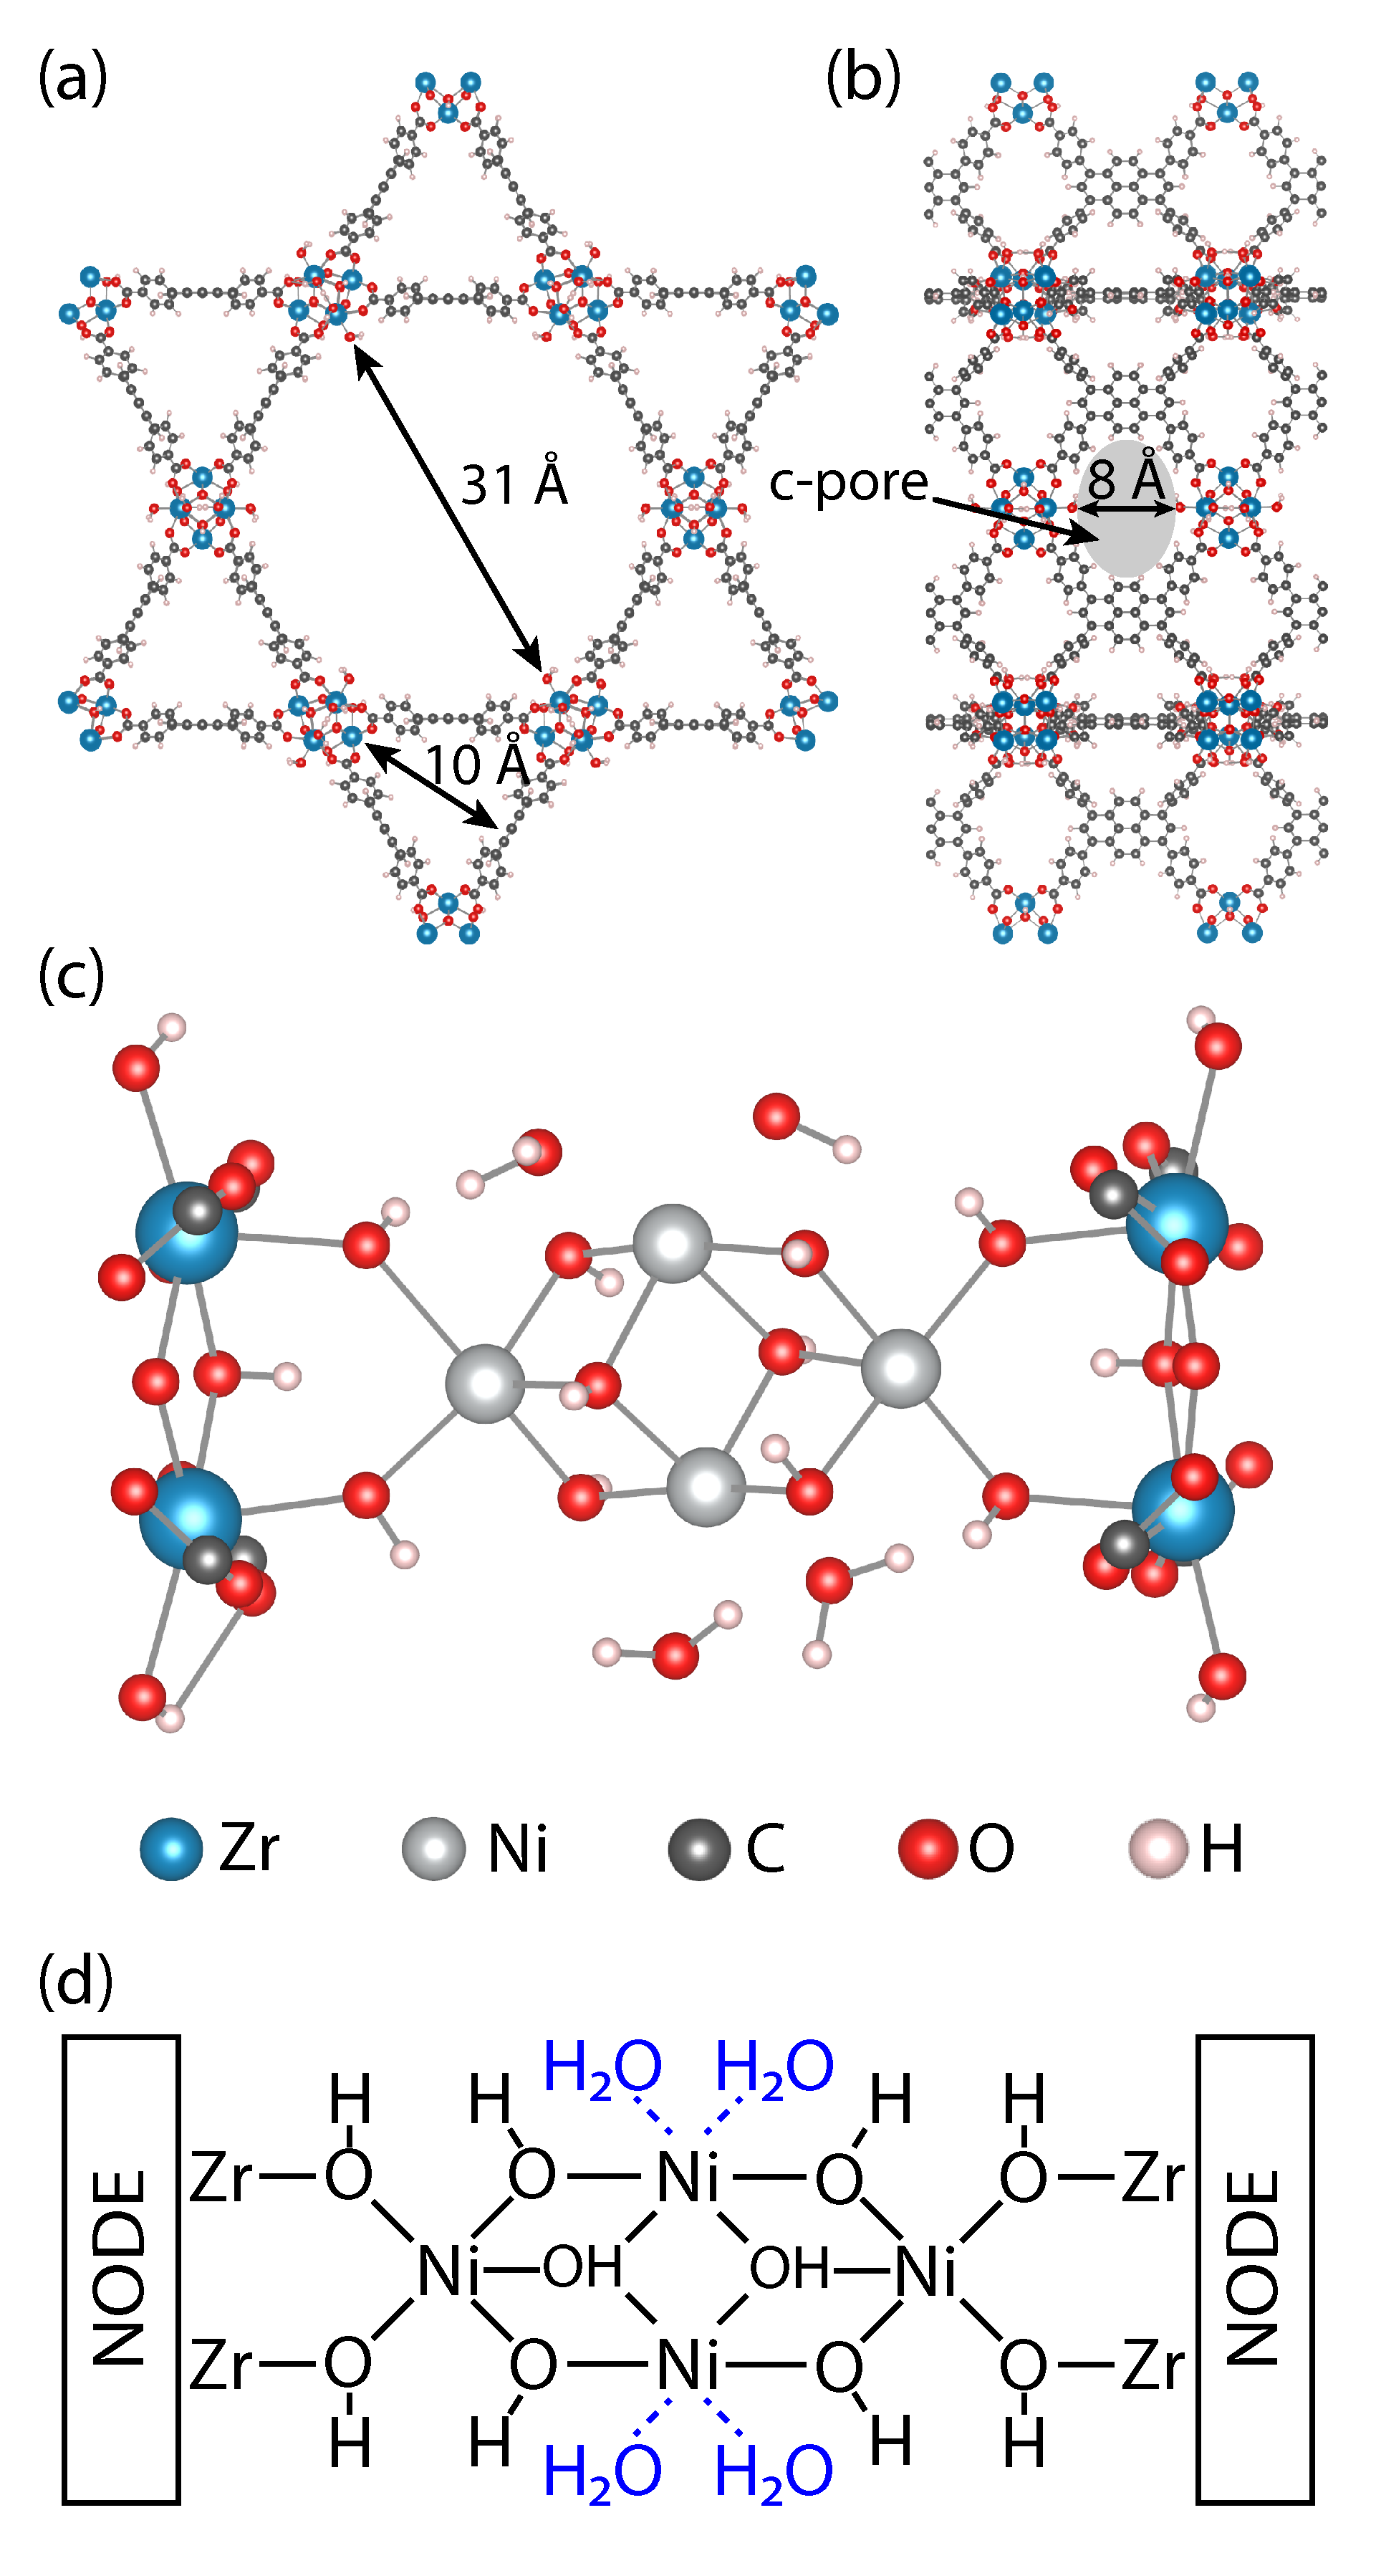
\includegraphics{zi-images/00-General-Graphics/2021-figure-MOF-structure.png}
    \caption{
    The structure of NU-1000 shown along the (a) c-axis and the (b) a-axis with the location of the metal complex location highlighted by the gray box. The proposed structure for the tetranuclear \ce{Ni} cluster is shown (c) atomistically and (d) schematically, with the MOF framework truncated from the renderings.}
    \label{fig:Ni-MOF-model}
\end{figure}

We select the \ce{Ni4(OH)6.4H2O} model, shown in Figure \ref{fig:Ni-MOF-model} \hl{(d) and (e)}, to be the reference structure for our investigation. While investigating how reaction conditions alter the catalyst structure, all structural and compositional transformations start from the \ce{Ni4(OH)6.4H2O} model, that is we explore the evolution of the composition and structure starting from the \ce{Ni4(OH)6.4H2O} model. Under \ce{H2}, both the \ce{Ni(II)} and \ce{OH} ligands provide sites that can accept dissociated \ce{H} atoms after \ce{H2} adsorption and dissociation. When these sites, defined as \ce{OH^{*}} and \ce{Ni^{*}}, accept dissociated \ce{H} atoms, the composition of the cluster changes to include additional adsorbed \ce{H2O} (\ce{H2O^{*}}) and/or Nickel-hydride (\ce{Ni-H}). However, the adsorbed \ce{H2O} are not fixed to the \ce{Ni} cluster; our modeling includes the subsequent desorption of \ce{H2O} into the gas-phase. All the aforementioned transformations are dependent on the reaction temperature ($T$), and \ce{H2} ($P_{\text{\ce{H2}}}$) and \ce{H2O} ($P_{\text{\ce{H2O}}}$) partial pressures. We model how the cluster structure and composition changes as a function of these different conditions by computing the free energy of compositionally different model structures  relative to a reference structure. We consider the chemical transformed described by the reversible reaction shown below (Equation \ref{eq:chemical-formula}):
\begin{equation}
    \begin{split}
        \ce{Ni4(OH)6.4H2O + xH2 (g) <=> Ni4(OH)_{10-(y+z)}(H)_{4+2x-(x+y)}.yH2O + zH2O (g)} \\
    \end{split}
    \label{eq:chemical-formula}
\end{equation}
where x defines the \ce{H2} added to the cluster, y is the number of adsorbed \ce{H2O} on the \ce{Ni} cluster, and z is the number of \ce{H2O} in the gas phase. We look at the thermodynamic stability of different modified clusters (\ce{Ni4(OH)_{10-(y+z)}(H)_{4+2x-(x+y)}}) that contain varying compositions of adsorbed (y) and gaseous (z) \ce{H2O} relative to the \ce{Ni4(OH)6.4H2O} model cluster. 

We generate a library of unique, modified structures by systematically adding \ce{H} atoms to the \ce{Ni^{*}} and \ce{OH^{*}} sites on the metal cluster. The \ce{H} addition process creates a new structure that is structurally and compositionally different from the reference structure. The new structure contains either \ce{Ni-H} or \ce{H2O^{*}}. The adsorbed \ce{H2O^{*}} is systematically removed thereby creating new structures. For these new structures, we again add \ce{H} atoms to the \ce{Ni^{*}} and \ce{OH^{*}} sites on the metal cluster and repeat the removal of any adsorbed \ce{H2O}. The iterative process creates a library of structures that are structurally and compositionally unique with \ce{H^{*}}, \ce{OH^{*}}, and \ce{Ni^{*}}. 

To determine the stability of the different structural and compositional variations for the \ce{Ni} metal complex, we calculate the relative free energy referenced to the \ce{Ni4(OH)6.4H2O} for each structure in library using \textit{ab initio} thermodynamic analysis. The approach requires a transformation of the free energy from a fixed number of atoms ($N_{\text{i}}$) to a fixed chemical potential ($\mu_{\text{i}}$). The free energy is transformed with respect to $\mu_{\text{H}^{*}}$, $\mu_{\text{OH}^{*}}$, and $\mu_{\text{Ni}^{*}}$ to account for structural and compositional variations in the number of adsorbed \ce{H} species ($N_{\text{H}^{*}}$), \ce{OH}-ligands ($N_{\text{OH}^{*}}$), and \ce{Ni} species ($N_{\text{Ni}^{*}}$). Equation \ref{eq:free-energy-trans} shows the free energy difference ($\Delta F^{(3)}(T,\mu_{\text{H}^{*}},\mu_{\text{OH}^{*}},\mu_{\text{Ni}^{*}})$) between structure $\text{j}$ and the \ce{Ni4(OH)6} reference structure (ref).
\begin{equation}
    \begin{split}
        \Delta F^{(3)}(T,\mu_{\text{H}^{*}},\mu_{\text{OH}^{*}},\mu_{\text{Ni}^{*}})  
        & = \Delta F^{(0)} - (\mu_{\text{H}^{*}})(\Delta N_{\text{H}^{*}}) \\ 
        & - (\mu_{\text{OH}^{*}})(\Delta N_{\text{OH}^{*}}) - (\mu_{\text{Ni}^{*}})(\Delta N_{\text{Ni}^{*}}) \\ 
    \end{split}
    \label{eq:free-energy-trans}
\end{equation}
The $\Delta F^{(0)}$ is the untransformed free energy difference between structure $\text{j}$ ($F_{\text{j}}$) and the reference structure ($F_{\text{ref}}$). The $F_{\text{j}}(T,N_{\text{j},\text{H}^{*}},N_{\text{j},\text{OH}^{*}},N_{\text{j},\text{Ni}^{*}})$ term is the free energy of structure $\text{j}$ with configuration of $N_{\text{j},\text{H}^{*}}$, $N_{\text{j},\text{OH}^{*}}$, and $N_{\text{j},\text{Ni}^{*}}$. We approximate the free energy ($F_{\text{j}}$) using the electronic energy from density functional theory (DFT). The $\Delta N$ terms are the difference between $N_{\text{j}}$ and $N_{\text{ref}}$ for each transformed species.

%We assume that $\ce{\text{H}^{*}}$ and $\ce{\text{OH}^{*}}$ are in equilibrium with an ideal-gas like reservoir with of %\ce{H2} and \ce{H2O}, respectively (as shown in Figure \ref{fig:FPT-process}). The chemical potential of the reservoir is %dependent on the reaction conditions ($T$ and $P$). The assumed equilibrium for $\ce{\text{H}^{*}}$ is with $\frac{1}{2}$ %\ce{H2} (g) and for $\ce{\text{OH}^{*}}$ is with \ce{H2O} (g)/$\frac{1}{2}$\ce{H2} (g) (Equation %\ref{eq:reaction_equilibrium}). The combined expression for $\ce{OH^{*}}$ captures the influence of both \ce{H2O} and %\ce{H2} gas phase conditions on the stability of the cluster (further details in the Supporting Information).
%\begin{equation}
%    \begin{split}
%        \frac{1}{2} H_{2} (g) & \ce{<=>} H^{*} \\           
%        \frac{1}{2} H_{2} (g) + OH^{*} & \ce{<=>} H_{2}O (g)  
%    \end{split}
%    \label{eq:reaction_equilibrium}
%\end{equation}
%Using Equation \ref{eq:reaction_equilibrium}, the relationship between the $\ce{\text{H}^{*}}$ and $\ce{OH^{*}}$ species %and the gas phase \ce{H2} and \ce{H2O} conditions are shown in Equation \ref{eq:chemicalpotentialeq}. The %$\mu_{i}^{g}(T,P)$ terms contain the temperature and pressure influences of the reaction conditions. 
%\begin{equation}
%    \begin{split}
%        \mu_{H^{*}} &= \frac{1}{2} \mu_{H_{2}}^{g}(T,P) \\ 
%        \mu_{OH^{*}} &= \mu_{H_{2}O}^{g}(T,P) - \frac{1}{2} \mu_{H_{2}}^{g}(T,P) \\
%    \end{split}
%    \label{eq:chemicalpotentialeq}
%\end{equation}

The chemical potential terms, $\mu_{\text{H}^{*}}$ and $\mu_{\text{OH}^{*}}$, include the temperature and pressure dependencies.\cite{Reuter2003,Reuter2004,Grundner2015,Paolucci2016,Li2016,Getman2008,Mandal2020}. We relate $\mu_{\text{H}^{*}}$ and $\mu_{\text{OH}^{*}}$ to $\mu_{\text{\ce{H2}}}^{\text{g}}(T,P)$ and $\mu_{\text{\ce{H2O}}}^{\text{g}}(T,P)$ by assuming each species is in equilibrium with an ideal gas-reservoir. The gas phase chemical potential terms, $\mu_{i}^{g}(T,P)$, are computed by correcting the electronic energy (referenced at $T$=0 K) of an isolated molecule with a chemical potential term, $\Delta \mu_{H_{2}}(T,P)$, that includes all the temperature- and pressure- dependent free-energy contributions (Equation \ref{eq:chemicalpotentialrel} ).
\begin{equation}
    \begin{split}
    \mu_{\text{i}}^{\text{g}}(T,P) &= E_{\text{i}} + \Delta \mu_{\text{i}}(T,P)  \\  
    \mu_{\text{i}}^{\text{g}}(T,P) &= E_{\text{i}} + \Big[ \Delta G_{\text{i}}(T,P^{o}) + RT \ln{\Big( \frac{P_{\text{i}}}{P^{o}} \Big)} \Big]  \\ 
    \end{split}
    \label{eq:chemicalpotentialrel}
\end{equation}
where $\text{i}$ represents either species \ce{H2} or \ce{H2O}. The gas-phase Gibbs free energies ($\Delta G_{\text{i}}(T,P^{o})$) at standard pressure ($P^{o}$) were computed using the NASA Polynomials\cite{Mcbride1993} in the pMuTT\cite{LYM2019106864} Python package. For \ce{Ni}, we approximate the chemical potential term ($\mu_{\text{Ni}^{*}}$) using the electronic energy of a bulk \ce{Ni} metal system. \hl{XXXX of the Supporting Information contains the full derivation for the \textit{ab initio} thermodynamic modeling approach.} 

We calculate $\mu_{\text{i}}^{\text{g}}(T,P)$ for both \ce{H2} and \ce{H2O} at temperatures ranging from 20 \degree C to 320 \degree C and \ce{H2} partial pressure ranging from $10^{-30}$ bar to $10^{5}$ bar at a fixed \ce{H2O} partial pressure of $10^{-9}$ bar. For each structure in the library, the free energy (Equation \ref{eq:free-energy-trans}) is calculated under range of activation conditions. For a given set of reaction conditions, we determined the most thermodynamically favorable structure by determining which structure minimizes the free energy (Equation \ref{eq:free-energy-trans}).  

The energies for the structures are from periodic density functional (DFT) calculations in CP2K.\cite{Hutter2014} The exchange correlation energy was calculated with the PBE functional\cite{Perdew1996} and corrected using damped D3 dispersion corrections formulated by \citeauthor{Grimme2010}.\cite{Grimme2010} The DZVP-MOLOPT basis set describes the valance electrons, Goedecker pseudopotentials\cite{Goedecker1996} describes the core electrons. The plane wave cutoff energy is 360 Ry and  all atoms in the periodic unit cell were allowed to relax during geometry optimizations (see Supporting information for a sample input file for further computational details). The variable spin states of the metal atoms required Unrestricted Kohn-Sham (UKS). For example, \ce{Ni(II)} can adopt both singlet (no unpaired electrons) and triplet (two unpaired electron) configurations. For clusters consisting of multiple \ce{Ni} atoms, we consider spin state permutations within the library of model structures. Any structures exhibiting spin contamination were removed from the analysis (see support information for more details).

\hl{How the PDFs are calculated from the model structures is something that is going to need to be included by Karena and Woodrow here.}

%%%%%%%%%%%%%%%%%%%%%%%%%%%%%%%%%%%%%%%%%%%%%%%%%%%%%%%%%%%%%%%%%%%%%
%% Results
%%%%%%%%%%%%%%%%%%%%%%%%%%%%%%%%%%%%%%%%%%%%%%%%%%%%%%%%%%%%%%%%%%%%%
\newpage
\section{Results}
Phase diagrams show the stability of structurally and compositionally different \ce{Ni} metal clusters as a function of different conditions. Each colored region on the phase diagrams corresponds to a different low energy structure based on the free energies values at those specific conditions. The free energies are calculated as a function of $T$ and $P_{\text{\ce{H2}}}$ at a fixed $P_{\text{\ce{H2O}}}=10^{-10}$ bar. Experimentally, the conditions the tetranuclear \ce{Ni(II)} cluster is exposed to do not contain any \ce{H2O} gas; therefore, we assume a small value for $P_{\text{\ce{H2O}}}$ as sufficient. The influence of $P_{\text{\ce{H2O}}}$ on the thermodynamic stability is shown in \hl{Figure XXXX within the Supporting Information}. 

\begin{figure}[H]
    \centering
    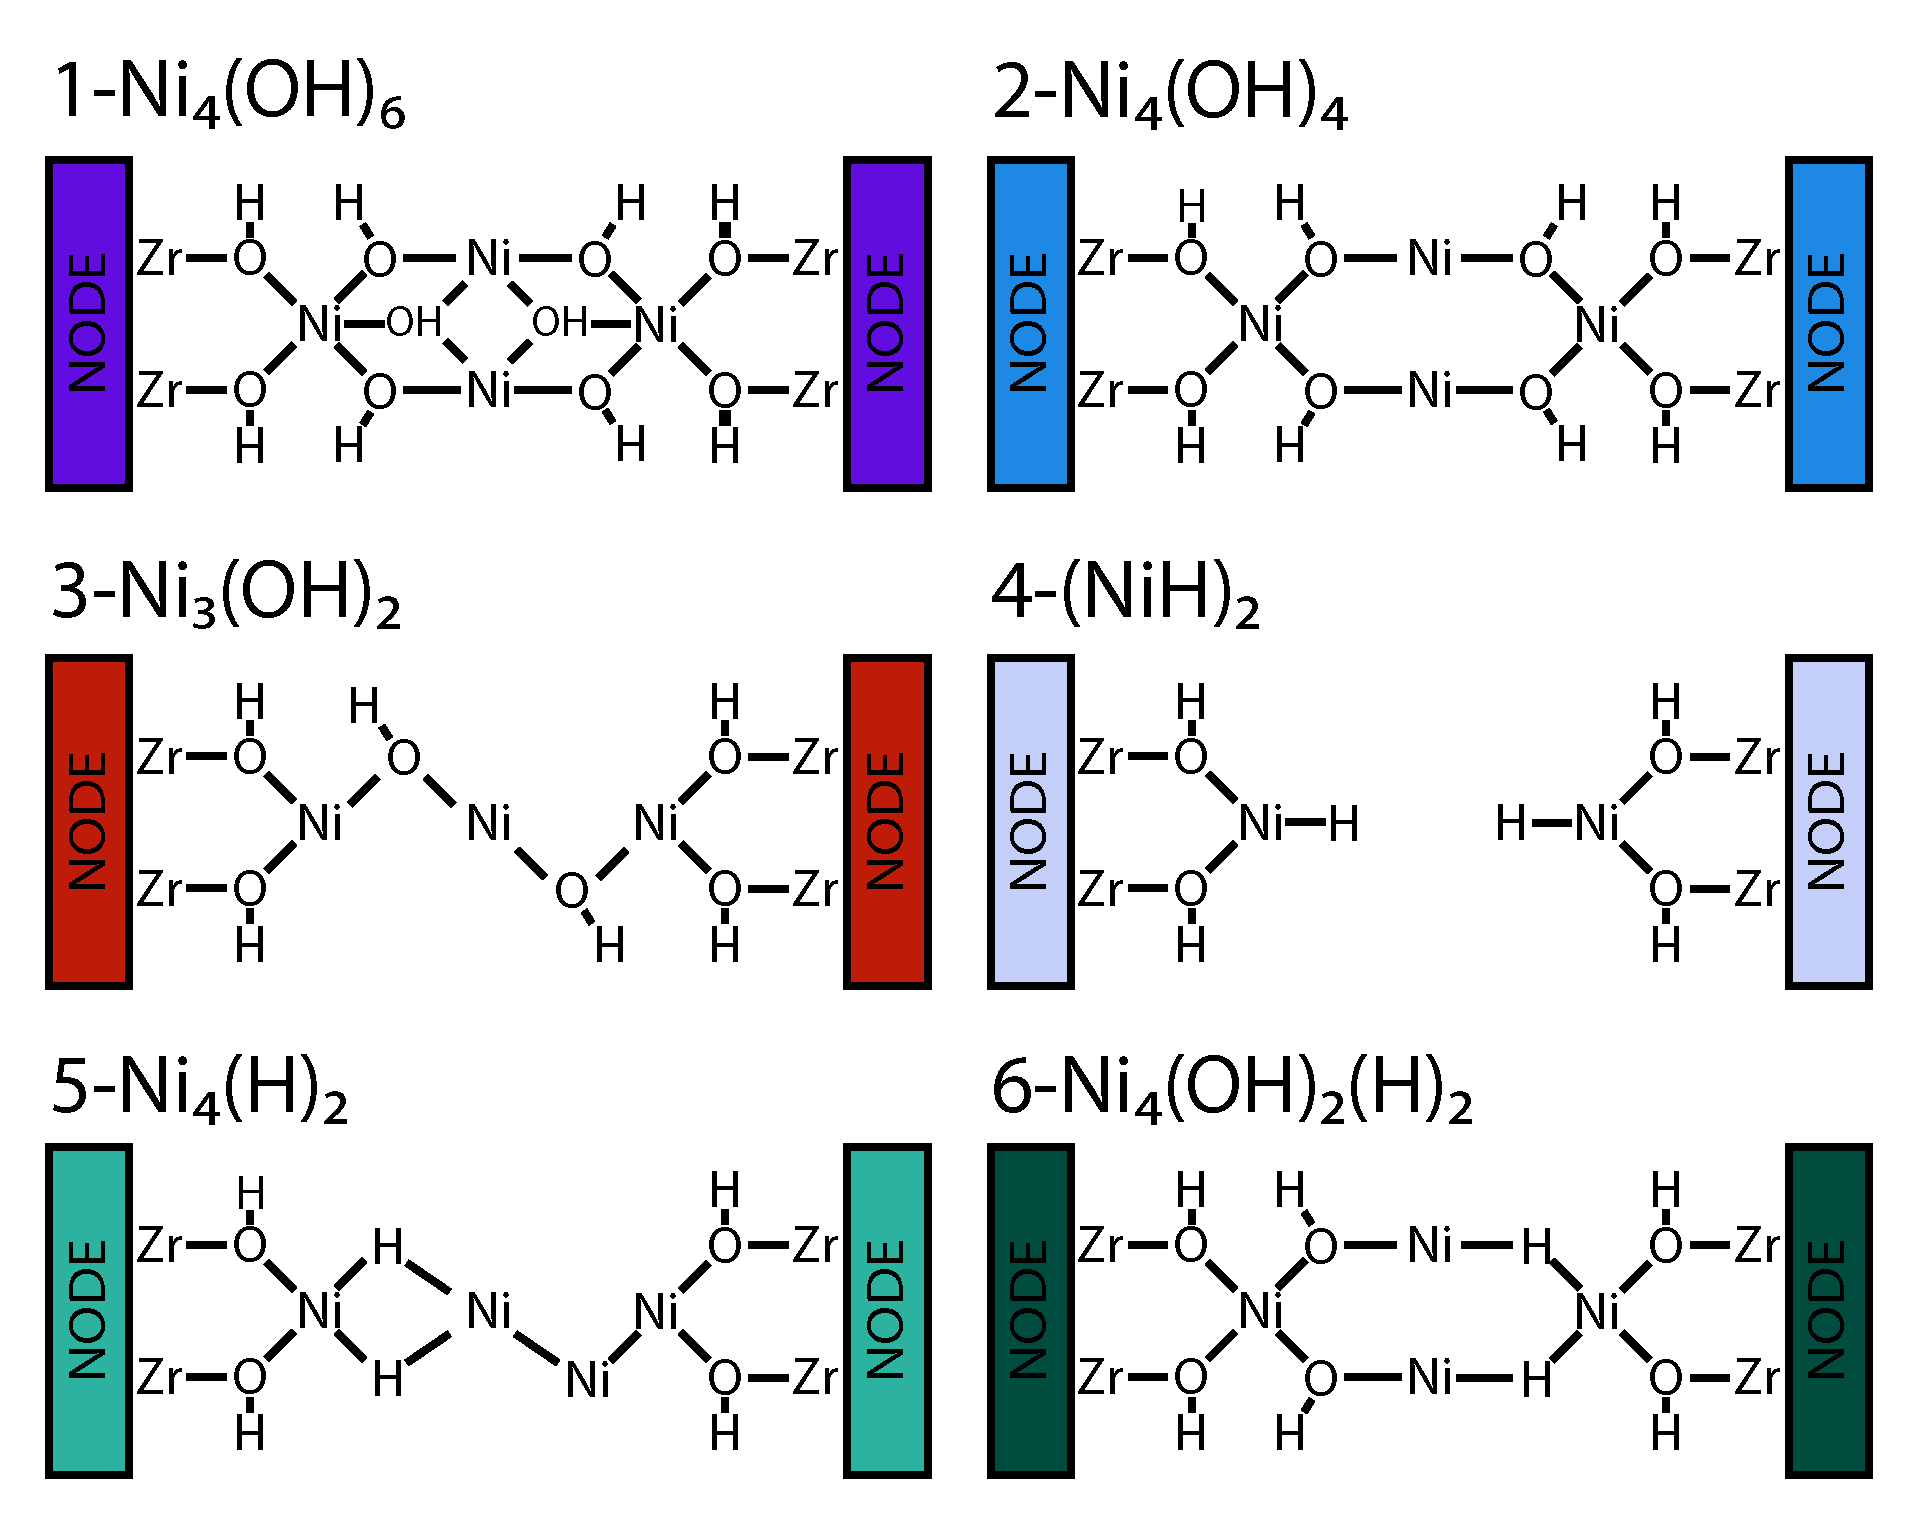
\includegraphics{zi-images/01-Ni-Graphics/2021-05-04--manuscript-structures.png}
    \caption{
    Schematic representation of key structures from the \textit{ab initio} thermodynamic analysis. Each structure minimize the free energy expression (Equation \ref{eq:free-energy-trans}) under some set of conditions explored during \textit{ab initio} thermodynamic analysis. A consistent naming convention and node coloring scheme is used in subsequent figures: 
        1-\ce{Ni4(OH)6} (purple),               % purple 
        2-\ce{Ni4(OH)4} (blue),                 % blue
        3-\ce{Ni3(OH)2} (red),                  % red 
        4-\ce{Ni2(H)2} (lilac),                 % lilac 
        5-\ce{Ni4(H)2} (mint), and              % mint
        6-\ce{Ni4(OH)2(H)2} (green).            % green
    }
    \label{fig:Ni-structure-diagram}
\end{figure}

The structures that minimize the free energy during \textit{ab initio} thermodynamic analysis are shown in Figure \ref{fig:Ni-structure-diagram}. The structural landscape of the \ce{Ni4} metal complex is diverse. Structurally and compositionally, the \ce{Ni} atoms contains a variable coordination sphere. The structures also exhibit a deviation in \ce{Ni} metal content from 2 to 4 \ce{Ni} atoms. Additionally, alternative structures that are thermodynamically relevant at higher $P_{\text{\ce{H2O}}}$ are located within the Supporting Information (\hl{see some part of the supporting information for these alternative conditions).} Figure \ref{fig:phase_diagram_Ni_combined} shows the relevant conditions for each structure at $P_{\text{\ce{H2O}}}=10^{-10}$ bar.

% The combined phase diagram figures
\begin{figure}[H]
    \centering
    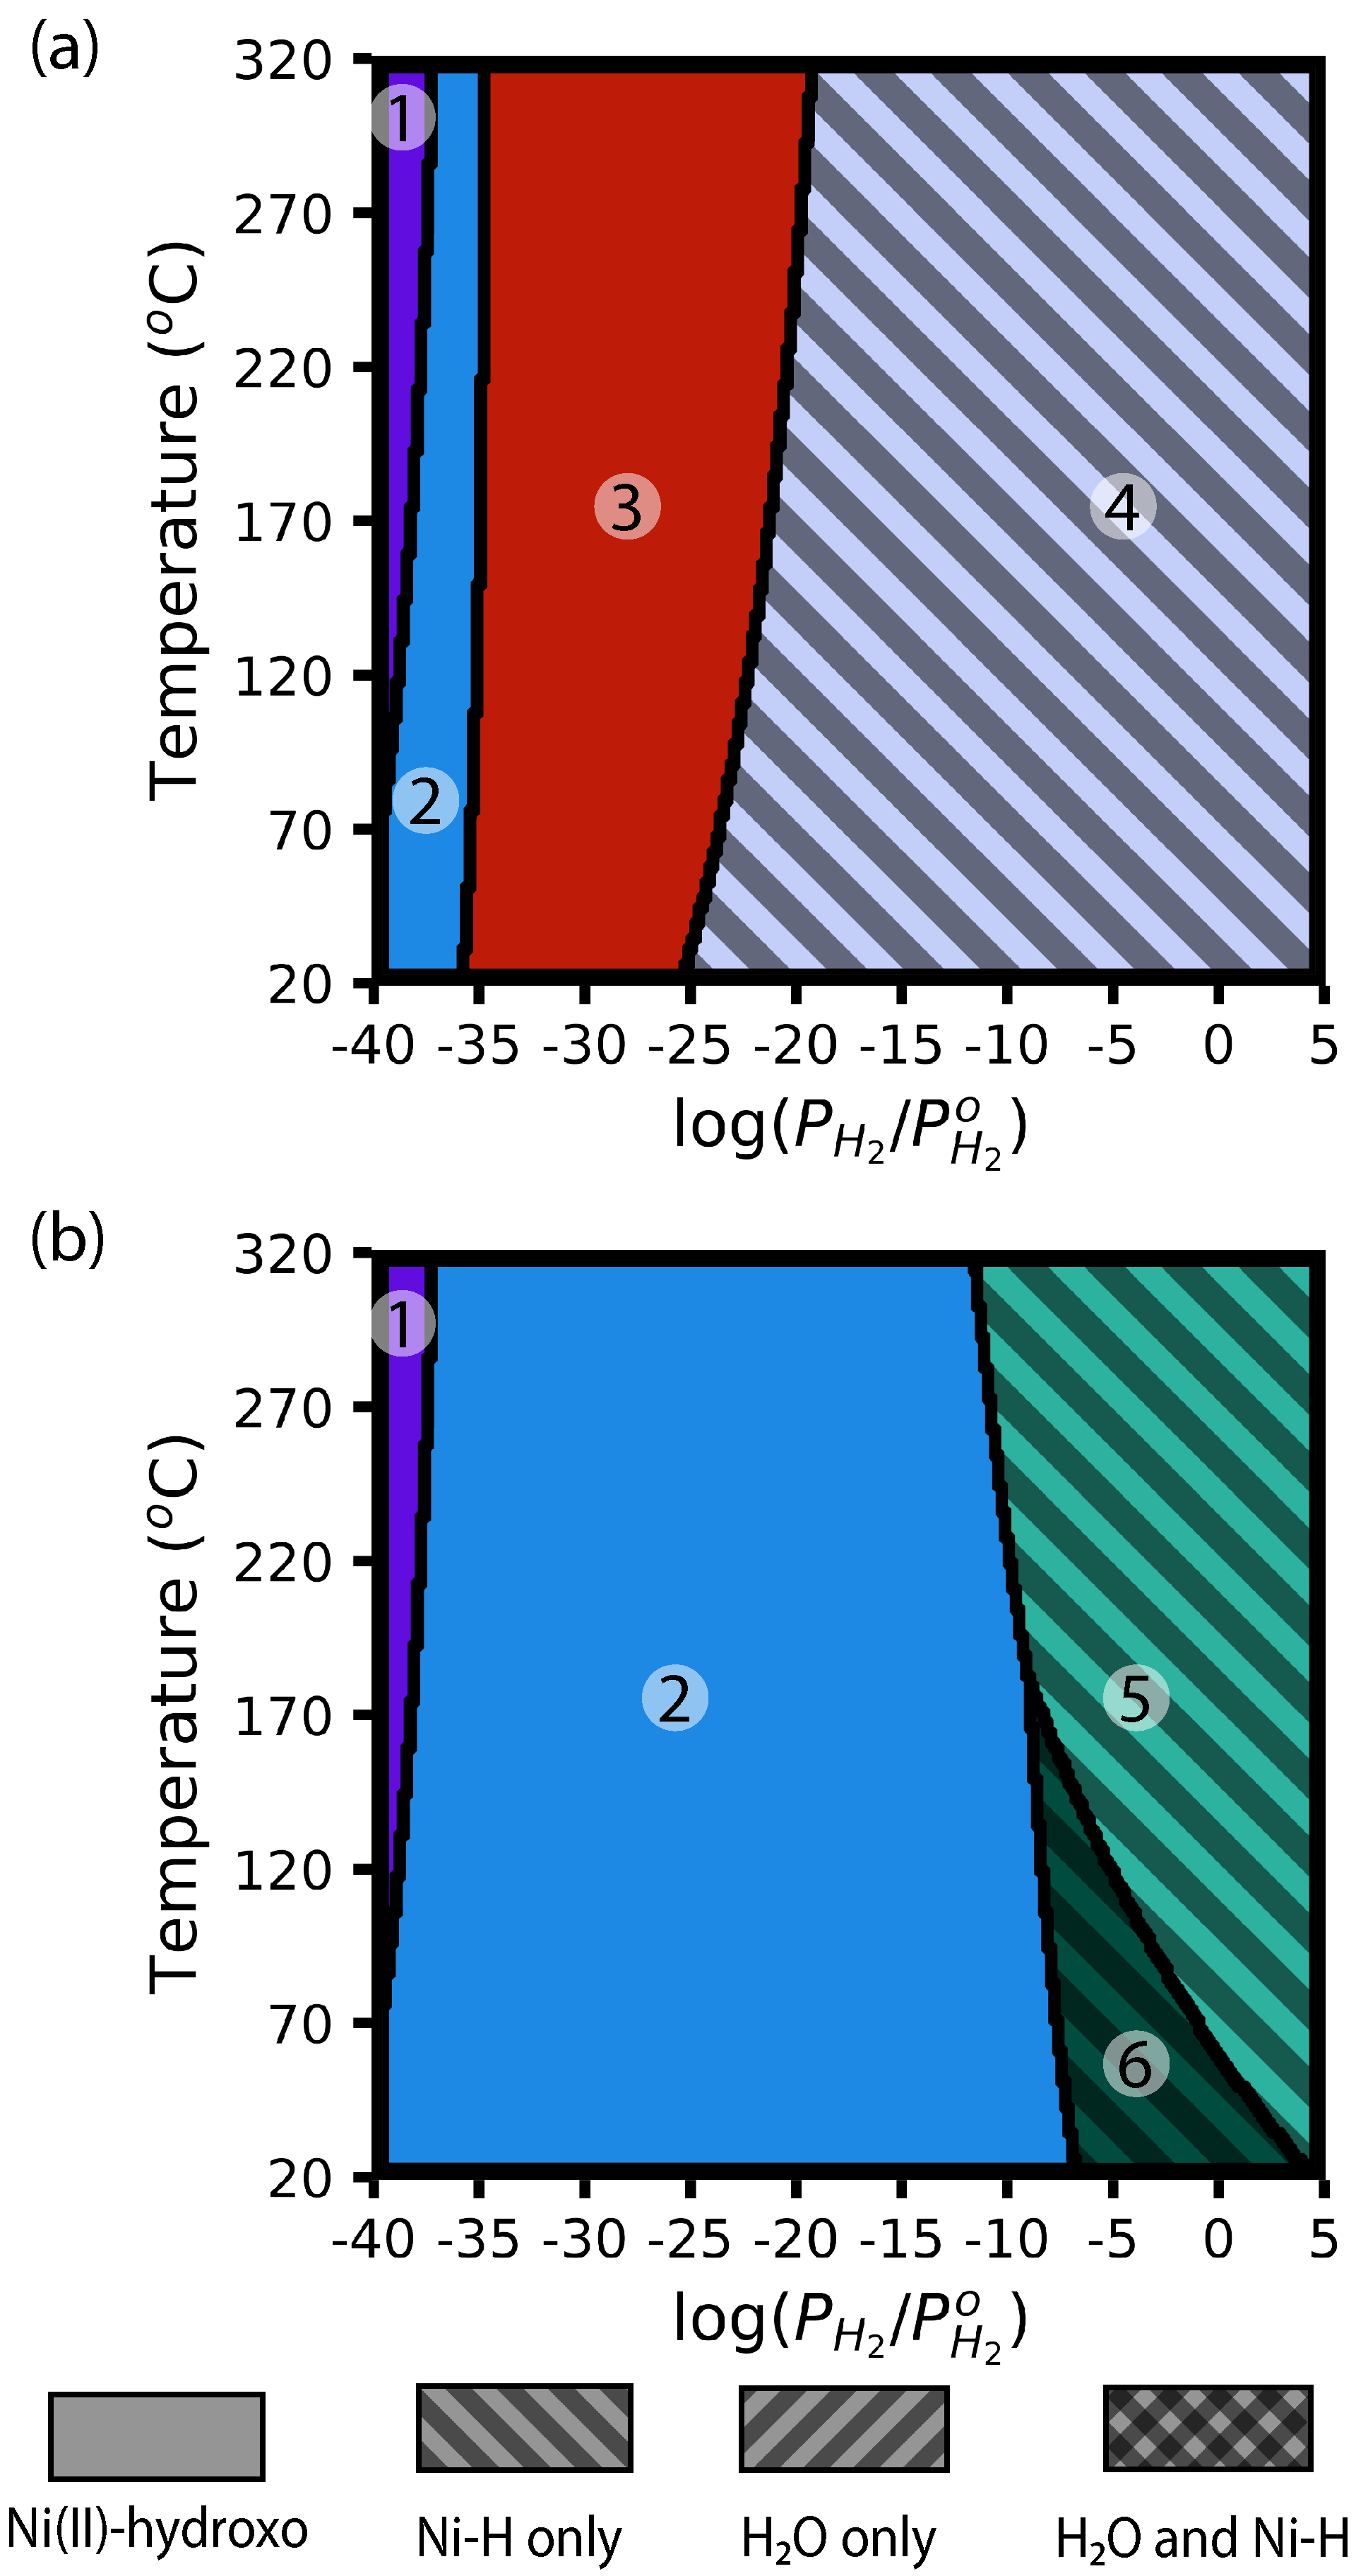
\includegraphics{zi-images/01-Ni-Graphics/2021-Ni-phase-diagram-combined.png}
    \caption{
    The stability of the \ce{Ni(II)} cluster as a function of temperature and \ce{H2} partial pressure at a \ce{H2O} partial pressure = $10^{-10}$ bar when transforming with (a) \ce{H^{*}}, \ce{OH^{*}}, and \ce{Ni^{*}} and, (b) \ce{H^{*}} and \ce{OH^{*}} (fixed \ce{Ni^{*}}). The colored regions indicate structures that minimize the free energy expression provided by Equation \ref{eq:free-energy-trans}. The interface between adjacent regions is denoted with black lines and correspond to where the free energy is equal between adjacent regions is equal. The \ce{H2} partial pressure is reported as $log(P_{\text{\ce{H2}}}/P_{\text{\ce{H2}}}^{o})$ and the standard pressure for both \ce{H2} ($P_{\text{\ce{H2}}}^{o}$) and \ce{H2O} ($P_{\text{\ce{H2O}}}^{o}$) is 1 bar. The following naming convention is adopted for the structures: 
        1-\ce{Ni4(OH)6} (purple),               % purple 
        2-\ce{Ni4(OH)4} (blue),                 % blue
        3-\ce{Ni3(OH)2} (red),                  % red 
        4-\ce{Ni2(H)2} (lilac),                 % lilac 
        5-\ce{Ni4(H)2} (mint), and              % mint
        6-\ce{Ni4(OH)2(H)2} (green).            % green
    }
    \label{fig:phase_diagram_Ni_combined}
\end{figure}   

The cluster is fully transformed, $\Delta F^{(3)}(T,\mu_{\text{H}^{*}},\mu_{\text{OH}^{*}},\mu_{\text{Ni}^{*}})$, in Figure \ref{fig:phase_diagram_Ni_combined} (a). With increasing \ce{H2} partial pressure, the $\ce{Ni^{*}}$ and $\ce{OH^{*}}$ composition of the cluster decreases. Lower \ce{H2} partial pressures favors 1-\ce{Ni4(OH)6} (purple) ($\ce{Ni^{*}}=4$, $\ce{OH^{*}}=6$, and $\ce{H^{*}}=0$) and shifts to 4-\ce{Ni2(H)2} (lilac) ($\ce{Ni^{*}}=2$, $\ce{OH^{*}}=0$, and $\ce{H^{*}}=2$) at higher \ce{H2} partial pressure. The transition between structures occurs via the transformation of \ce{OH}-ligands into \ce{H2O} because of the increasing \ce{H2} partial pressure. Figure \ref{fig:phase_diagram_Ni_combined} (a) suggests that the cluster stability is a more dependent on \ce{H2} partial pressure than temperature. Also, we further evaluate the removal of the entire complex, which revealed that under the conditions shown in Figure \ref{fig:phase_diagram_Ni_combined} (a) that the global thermodynamic minimum is the NU-1000 MOF support without any \ce{Ni} supported metal complex. This suggests that the \ce{Ni} metal cluster is in a metastable state that is ultimately driven towards nanoparticle formation. 

We evaluate the performance of our model by comparing the model dPDFs to experimental dPDFs for an activated \ce{Ni} metal complex supported on NU-1000. The synthesized tetranuclear \ce{Ni} cluster exposed to \ce{H2} (3.5\% in \ce{He}) at 200 \degree C for 2 hours and then cooled to 50 \degree C in \ce{H2}.\cite{PlateroPrats2017} Powder X-ray diffraction (XRD) and total scattering data suitable for PDF analysis were collected at 50 \degree C in \ce{H2}. The dPDFs provide structural insights into the cluster by revealing key interatomic distances with peaks indicating the distance between different atoms. Experimentally, the significant dPDF peaks are the \ce{Ni-O} bond length at 2.02 {\AA}, the \ce{Ni{\Compactcdots}Ni} distances at 3.01 {\AA} and 3.27 {\AA}, and the \ce{Ni{\Compactcdots}Zr} distances at 3.78 {\AA} and 4.08 {\AA}. The experimental, activated dPDFs for \ce{Ni{\Compactcdots}Ni} and \ce{Ni{\Compactcdots}Zr} contain multiple peaks that suggests asymmetric distances within the cluster. Figure \ref{fig:dPDFs_TandP_trans_Ni} shows the dPDFs for all the thermodynamically favorable structures found in Figure \ref{fig:phase_diagram_Ni_combined}.

% dPDF diagram for the phase diagram structures 
\begin{figure}[H]
    \centering
    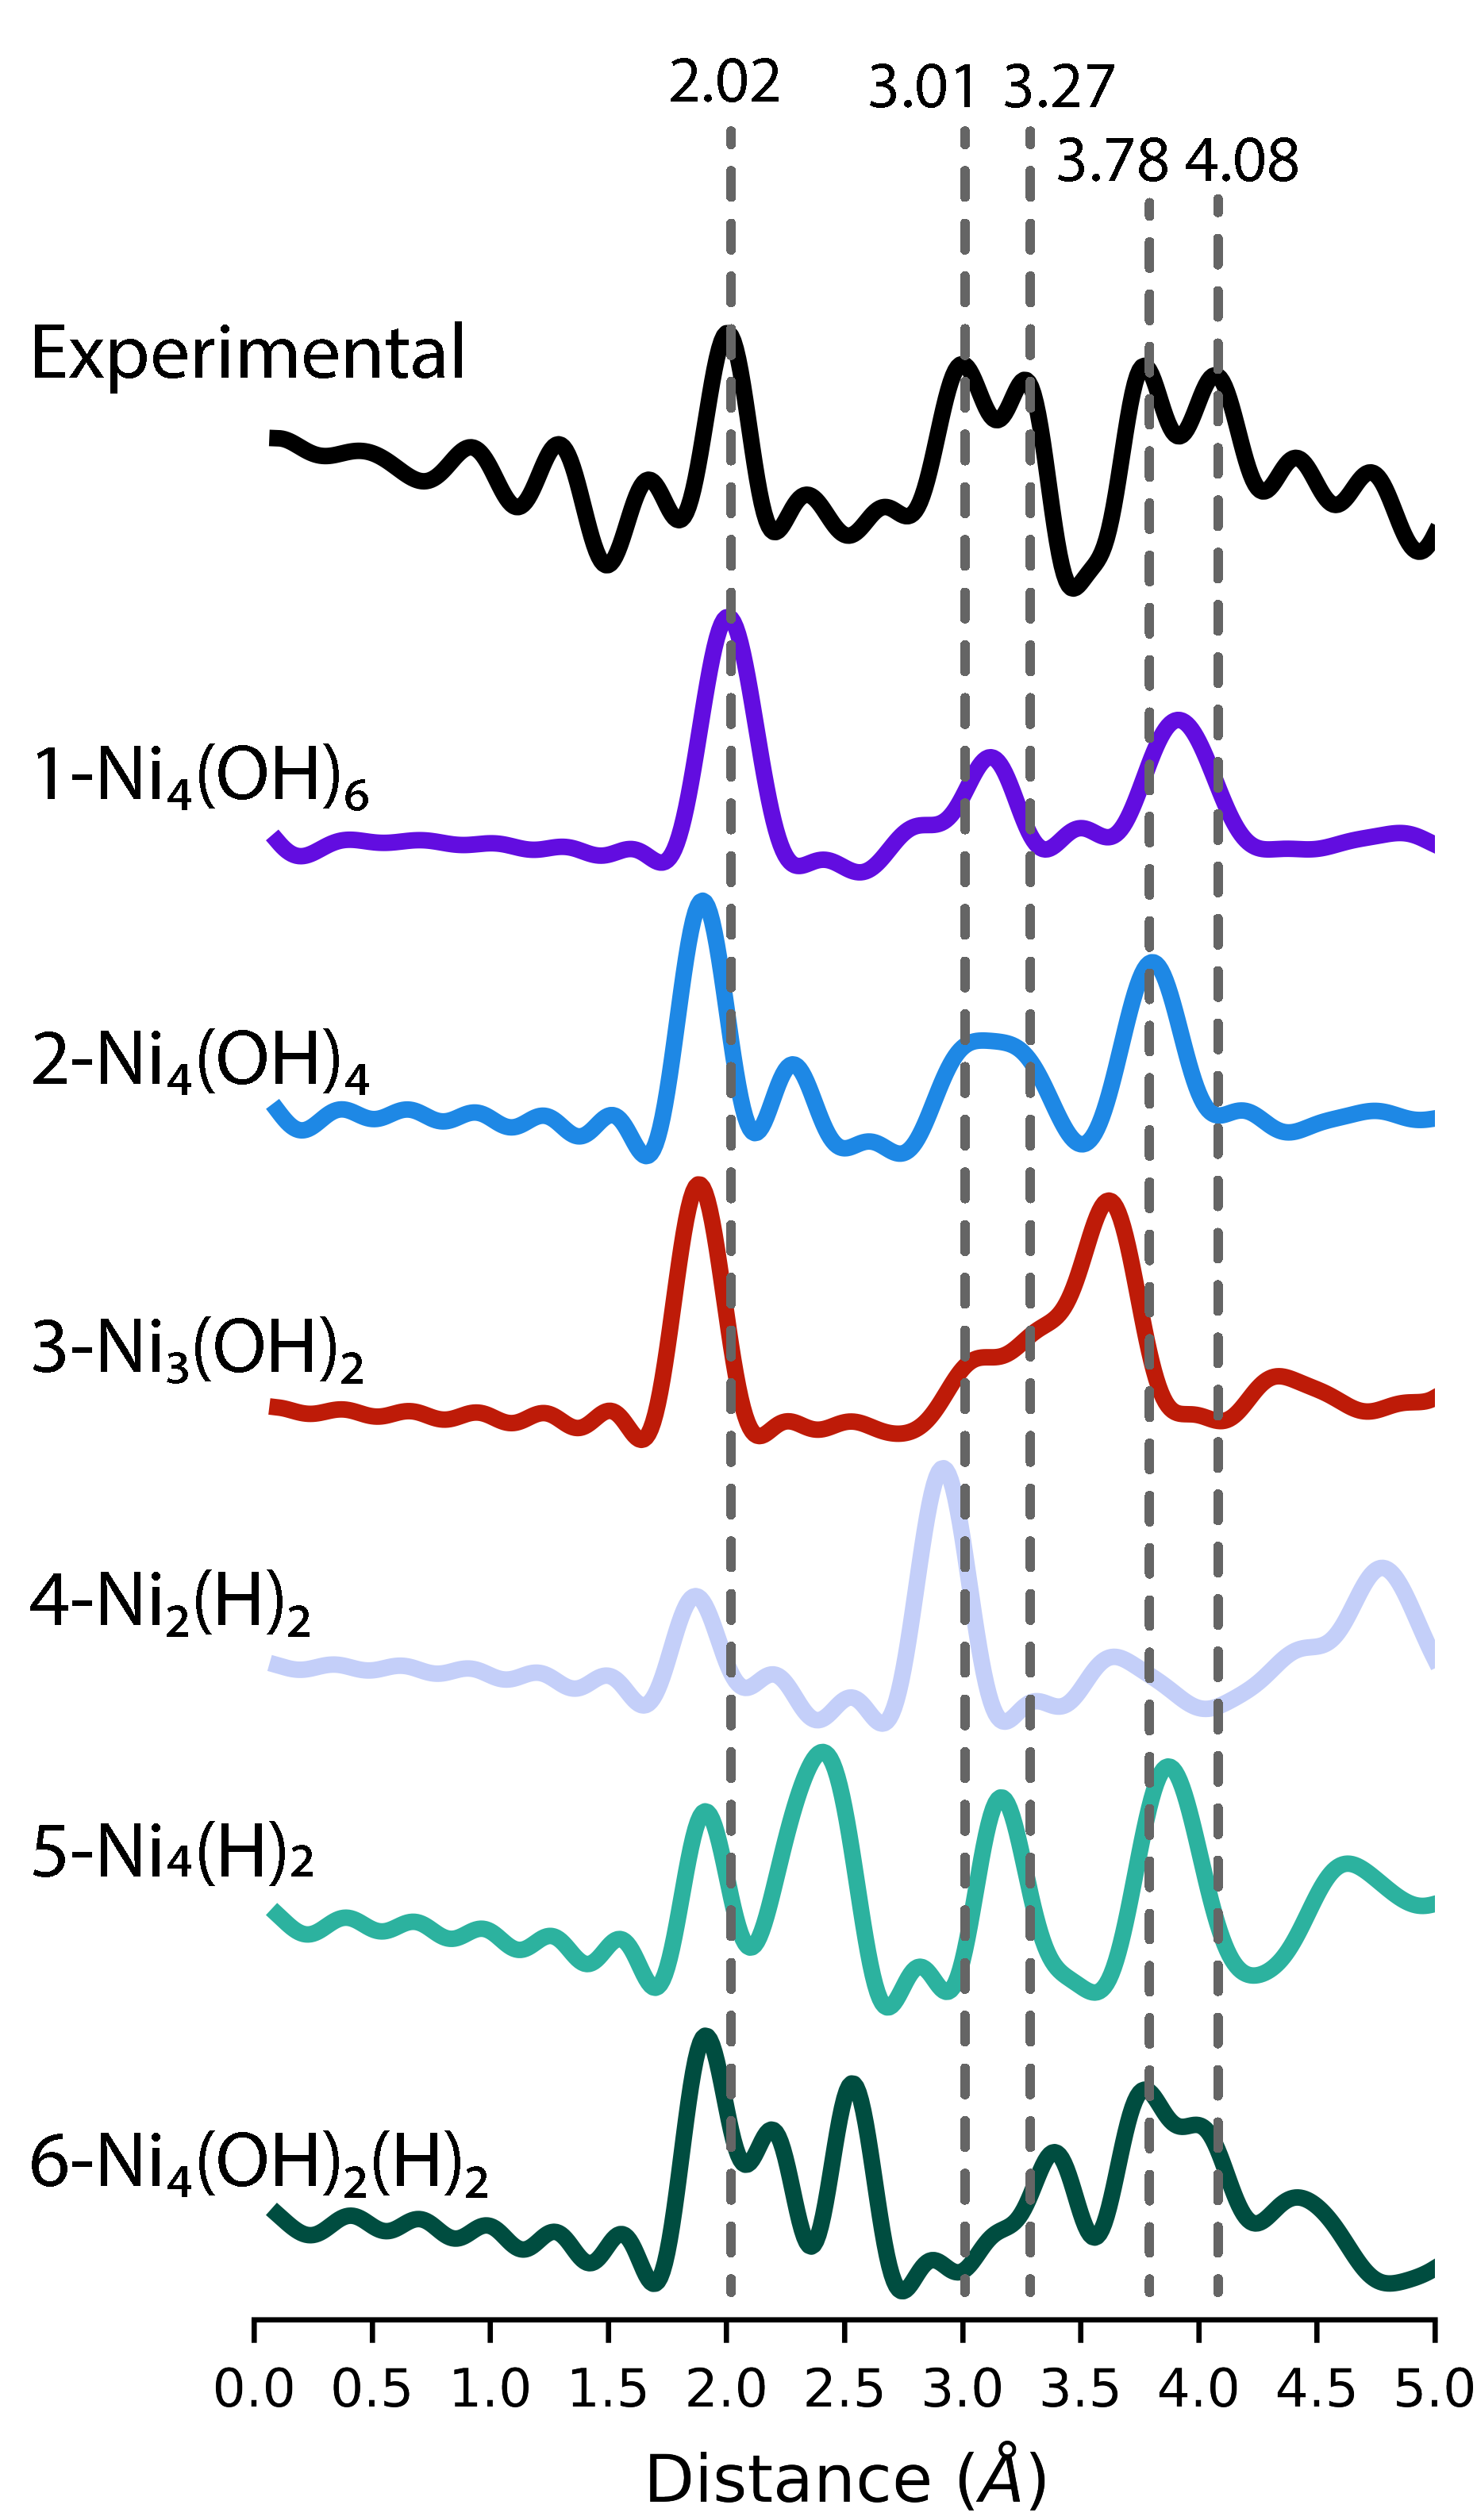
\includegraphics{zi-images/01-Ni-Graphics/2021-MAIN-single-dPDF-phase-diagram.png}
    \caption{
    Differential pair distribution functions (dPDFs) for all the activated structures, using the same color scheme from the \ce{Ni(II)} phase diagram shown in Figure \ref{fig:phase_diagram_Ni_combined}. Analyzing the peak positions provide a metric to evaluate the local structure of the model structures in comparison to the experimental. 
    }
    \label{fig:dPDFs_TandP_trans_Ni}
\end{figure}

Figure \ref{fig:dPDFs_TandP_trans_Ni} features four structures that are thermodynamically relevant under the explore conditions: 1-\ce{Ni4(OH)6} (purple), 2-\ce{Ni4(OH)4} (blue), 3-\ce{Ni3(OH)2} (red), and 4-\ce{Ni2(H)2} (lilac). The \ce{Ni-O} peak at 2.02 {\AA} is matched by  1-\ce{Ni4(OH)6} (purple), but underpredicted by 2-\ce{Ni4(OH)4} (blue), 3-\ce{Ni3(OH)2} (red), and 4-\ce{Ni2(H)2} (lilac). For the \ce{Ni{\Compactcdots}Ni} peaks, both  1-\ce{Ni4(OH)6} (purple) and  2-\ce{Ni4(OH)4} (blue) exhibit a single peak within the experimental bounds of 3.01 {\AA} and 3.27 {\AA}. Structure 3-\ce{Ni3(OH)2} (red) features a poorly defined back at 3.11 {\AA} attributed to a \ce{Ni{\Compactcdots}Ni} peak meanwhile 4-\ce{Ni2(H)2} (lilac) has no \ce{Ni{\Compactcdots}Ni} peak. For the \ce{Ni{\Compactcdots}Zr} peaks, both  1-\ce{Ni4(OH)6} (purple) and 2-\ce{Ni4(OH)4} (blue) again exhibit a single peak within the experimental bounds of 3.78 {\AA} and 4.08 {\AA}. 3-\ce{Ni3(OH)2} (red) has a \ce{Ni{\Compactcdots}Zr} peak at 3.63 {\AA} and 4-\ce{Ni2(H)2} (lilac) exhibits a single \ce{Ni{\Compactcdots}Zr} peak at 2.93 {\AA}.

For the thermodynamically relevant structures from Figure \ref{fig:phase_diagram_Ni_combined} (a), only structures 1-\ce{Ni4(OH)6} (purple) and 2-\ce{Ni4(OH)4} (blue) show reasonable agreement when compared to the experimental dPDF. However, both of these structures fail to recreate the experimental peak splitting for \ce{Ni{\Compactcdots}Ni} and \ce{Ni{\Compactcdots}Zr}. Additionally, 2-\ce{Ni4(OH)4} demonstrates an additional \ce{Ni{\Compactcdots}Ni} peak at 2.29 {\AA}. The difference between 1-\ce{Ni4(OH)6} (purple) and 2-\ce{Ni4(OH)4} compared to 3-\ce{Ni3(OH)2} (red) and 4-\ce{Ni2(H)2} (lilac) is the difference in \ce{Ni} coordination environment with the latter have a low coordination number. The structures that are less coordinated shown in Figure \ref{fig:Ni-structure-diagram} fail to match the experimentally observed coordination environment for the \ce{Ni} atoms. We illustrate the findings of \citeauthor{PlateroPrats2017} that the \ce{Ni} metal cluster features a higher \ce{Ni} coordination (approximately 5) environment. 

Given that structures with \ce{Ni} content less than 4 \ce{Ni} fail to recreate the experimental peak positions, we impose a constraint on our model to only transform with $\ce{H^{*}}$ and $\ce{OH^{*}}$. By no longer transforming with $\ce{Ni^{*}}$, we maintain a constant \ce{Ni} composition and repeat the \textit{ab initio} thermodynamic analysis. Figure \ref{fig:phase_diagram_Ni_combined} (b) shows the thermodynamic stability of the cluster when transforming with respect to composition of $\ce{H^{*}}$ and $\ce{OH^{*}}$ at a fixed \ce{Ni^{*}} composition. 1-\ce{Ni4(OH)6} (purple) and 2-\ce{Ni4(OH)4} (blue) appear on both Figure \ref{fig:phase_diagram_Ni_combined} (a) and (b). The new structures appear appearing on \ref{fig:phase_diagram_Ni_combined} (b) are 5-\ce{Ni4(H)2} (mint) and 6-\ce{Ni4(OH)2(H)2} (green).

We now focus on the dPDFs for 5-\ce{Ni4(H)2} (mint) and 6-\ce{Ni4(OH)2(H)2} (green) (Figure \ref{fig:dPDFs_TandP_trans_Ni}). Similar to our previous discussion, we observe that both 5-\ce{Ni4(H)2} (mint) and 6-\ce{Ni4(OH)2(H)2} (green) underpredict the \ce{Ni-O} peak. Both 5-\ce{Ni4(H)2} (mint) and 6-\ce{Ni4(OH)2(H)2} (green) show good agreement with the \ce{Ni{\Compactcdots}Zr} peaks, with 6-\ce{Ni4(OH)2(H)2} (green) showing the split \ce{Ni{\Compactcdots}Zr} peaks that are experimentally observed. For the \ce{Ni{\Compactcdots}Ni} peaks, only 5-\ce{Ni4(H)2} (mint) contains a peak within the experimental bounds of the split \ce{Ni{\Compactcdots}Ni} peaks. However, both 5-\ce{Ni4(H)2} (mint) and 6-\ce{Ni4(OH)2(H)2} (green) contain sharp \ce{Ni{\Compactcdots}Ni} peaks at 2.42 and 2.54 {\AA}, respectively. 6-\ce{Ni4(OH)2(H)2} also contains a \ce{Ni{\Compactcdots}Ni} peak 2.20 {\AA}. The presence of these additional \ce{Ni{\Compactcdots}Ni} peaks for 5-\ce{Ni4(H)2} (mint) and 6-\ce{Ni4(OH)2(H)2} (green) suggests that both of these structures are not closely related to the experimental structure. Again, we observe that structures 5-\ce{Ni4(H)2} (mint) and 6-\ce{Ni4(OH)2(H)2} (green) underpredict the \ce{Ni} coordination environment.

Our analysis therefore suggests that even at increased temperatures and exposure to \ce{H2} gas, the cluster must remain highly ordered. To further evaluate our model and better understand the \ce{Ni} active site structure, we search the model structure library to find structures that more closely match the peak splitting observed experimental and \ce{Ni} coordination environment. Our search consisted of both increasing the \ce{H2O} partial pressure to generate phase diagrams with a higher \ce{Ni} coordination environment (\hl{supporting information XXX}) and inspecting the \ce{Ni-O}, \ce{Ni{\Compactcdots}Ni}, and \ce{Ni{\Compactcdots}Zr} distances of structures that are not thermodynamic minimum from \textit{ab initio} thermodynamic analysis. 

\begin{figure}[H]
    \centering
    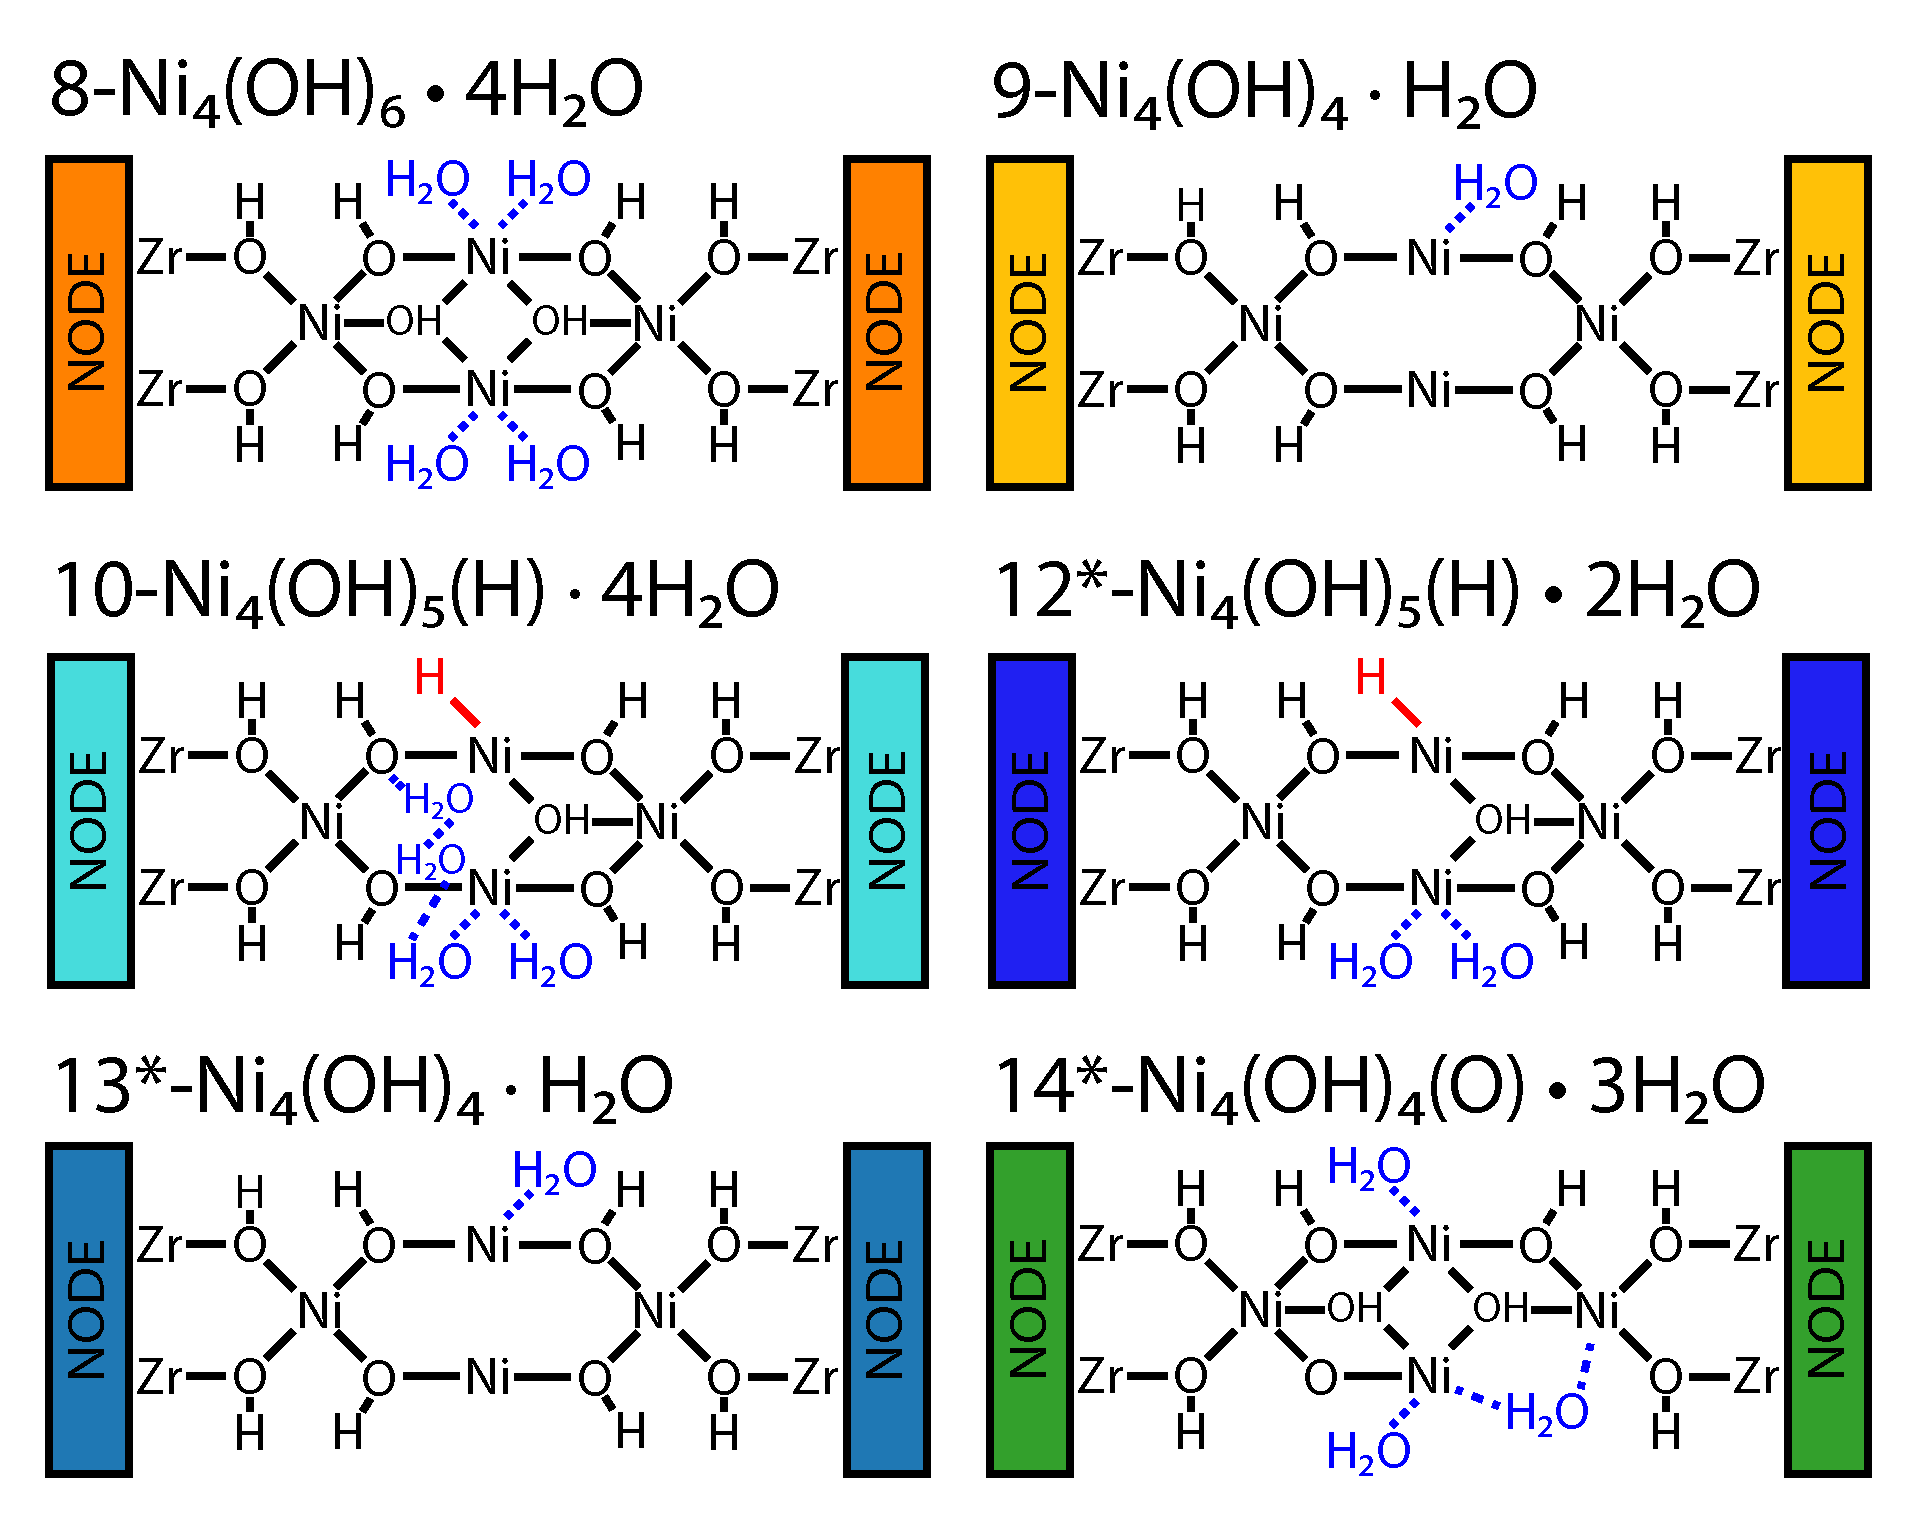
\includegraphics{zi-images/01-Ni-Graphics/2021-05-06--manuscript-structures-select.png}
    \caption{
        Schematic representation of structures from \textit{ab initio} thermodynamic analysis at higher \ce{H2O} partial pressures and select structure based on \ce{Ni-O}, \ce{Ni{\Compactcdots}Ni}, and \ce{Ni{\Compactcdots}Zr} atomic distances. The select structures are not thermodynamic minimum under any explored conditions and are denoted using a * (for example, 12*-\ce{Ni4(OH)5(H).2H2O} (royal)). A consistent naming convention and node coloring scheme is used in subsequent figures: 
            8-\ce{Ni4(OH)6.4H2O} (orange),        
            9-\ce{Ni4(OH)4.H2O} (yellow),         
            10-\ce{Ni4(OH)5(H).4H2O} (teal),      
            12*-\ce{Ni4(OH)5(H).2H2O} (royal),
            13*-\ce{Ni4(OH)6.H2O} (blue), and 
            14*-\ce{Ni4(OH)4(O).3H2O} (green)
    }
    \label{fig:Ni-structure-diagram-select}
\end{figure}

Our research revealed six structures (Figure \ref{fig:Ni-structure-diagram-select}) that include a high \ce{Ni} coordination and interesting dPDF peaks. The structures include our initial reference structure (8-\ce{Ni4(OH)6.4H2O} (orange)), structures similar to 2-\ce{Ni4(OH)4} (blue) that now contain an absorbed \ce{H2O} (9-\ce{Ni4(OH)4.H2O} (yellow) and 13*-\ce{Ni4(OH)6.H2O} (blue)), and three unique structures that contain additional coordinated \ce{H2O} (10-\ce{Ni4(OH)5(H).4H2O} (teal), 12*-\ce{Ni4(OH)5(H).2H2O} (royal), and 14*-\ce{Ni4(OH)4(O).3H2O} (green)). We compare the local structure of the experimental dDPF to the structure dPDFs for each in Figure \ref{fig:dPDFs_TandP_trans_Ni-select}

\begin{figure}[H]
    \centering
    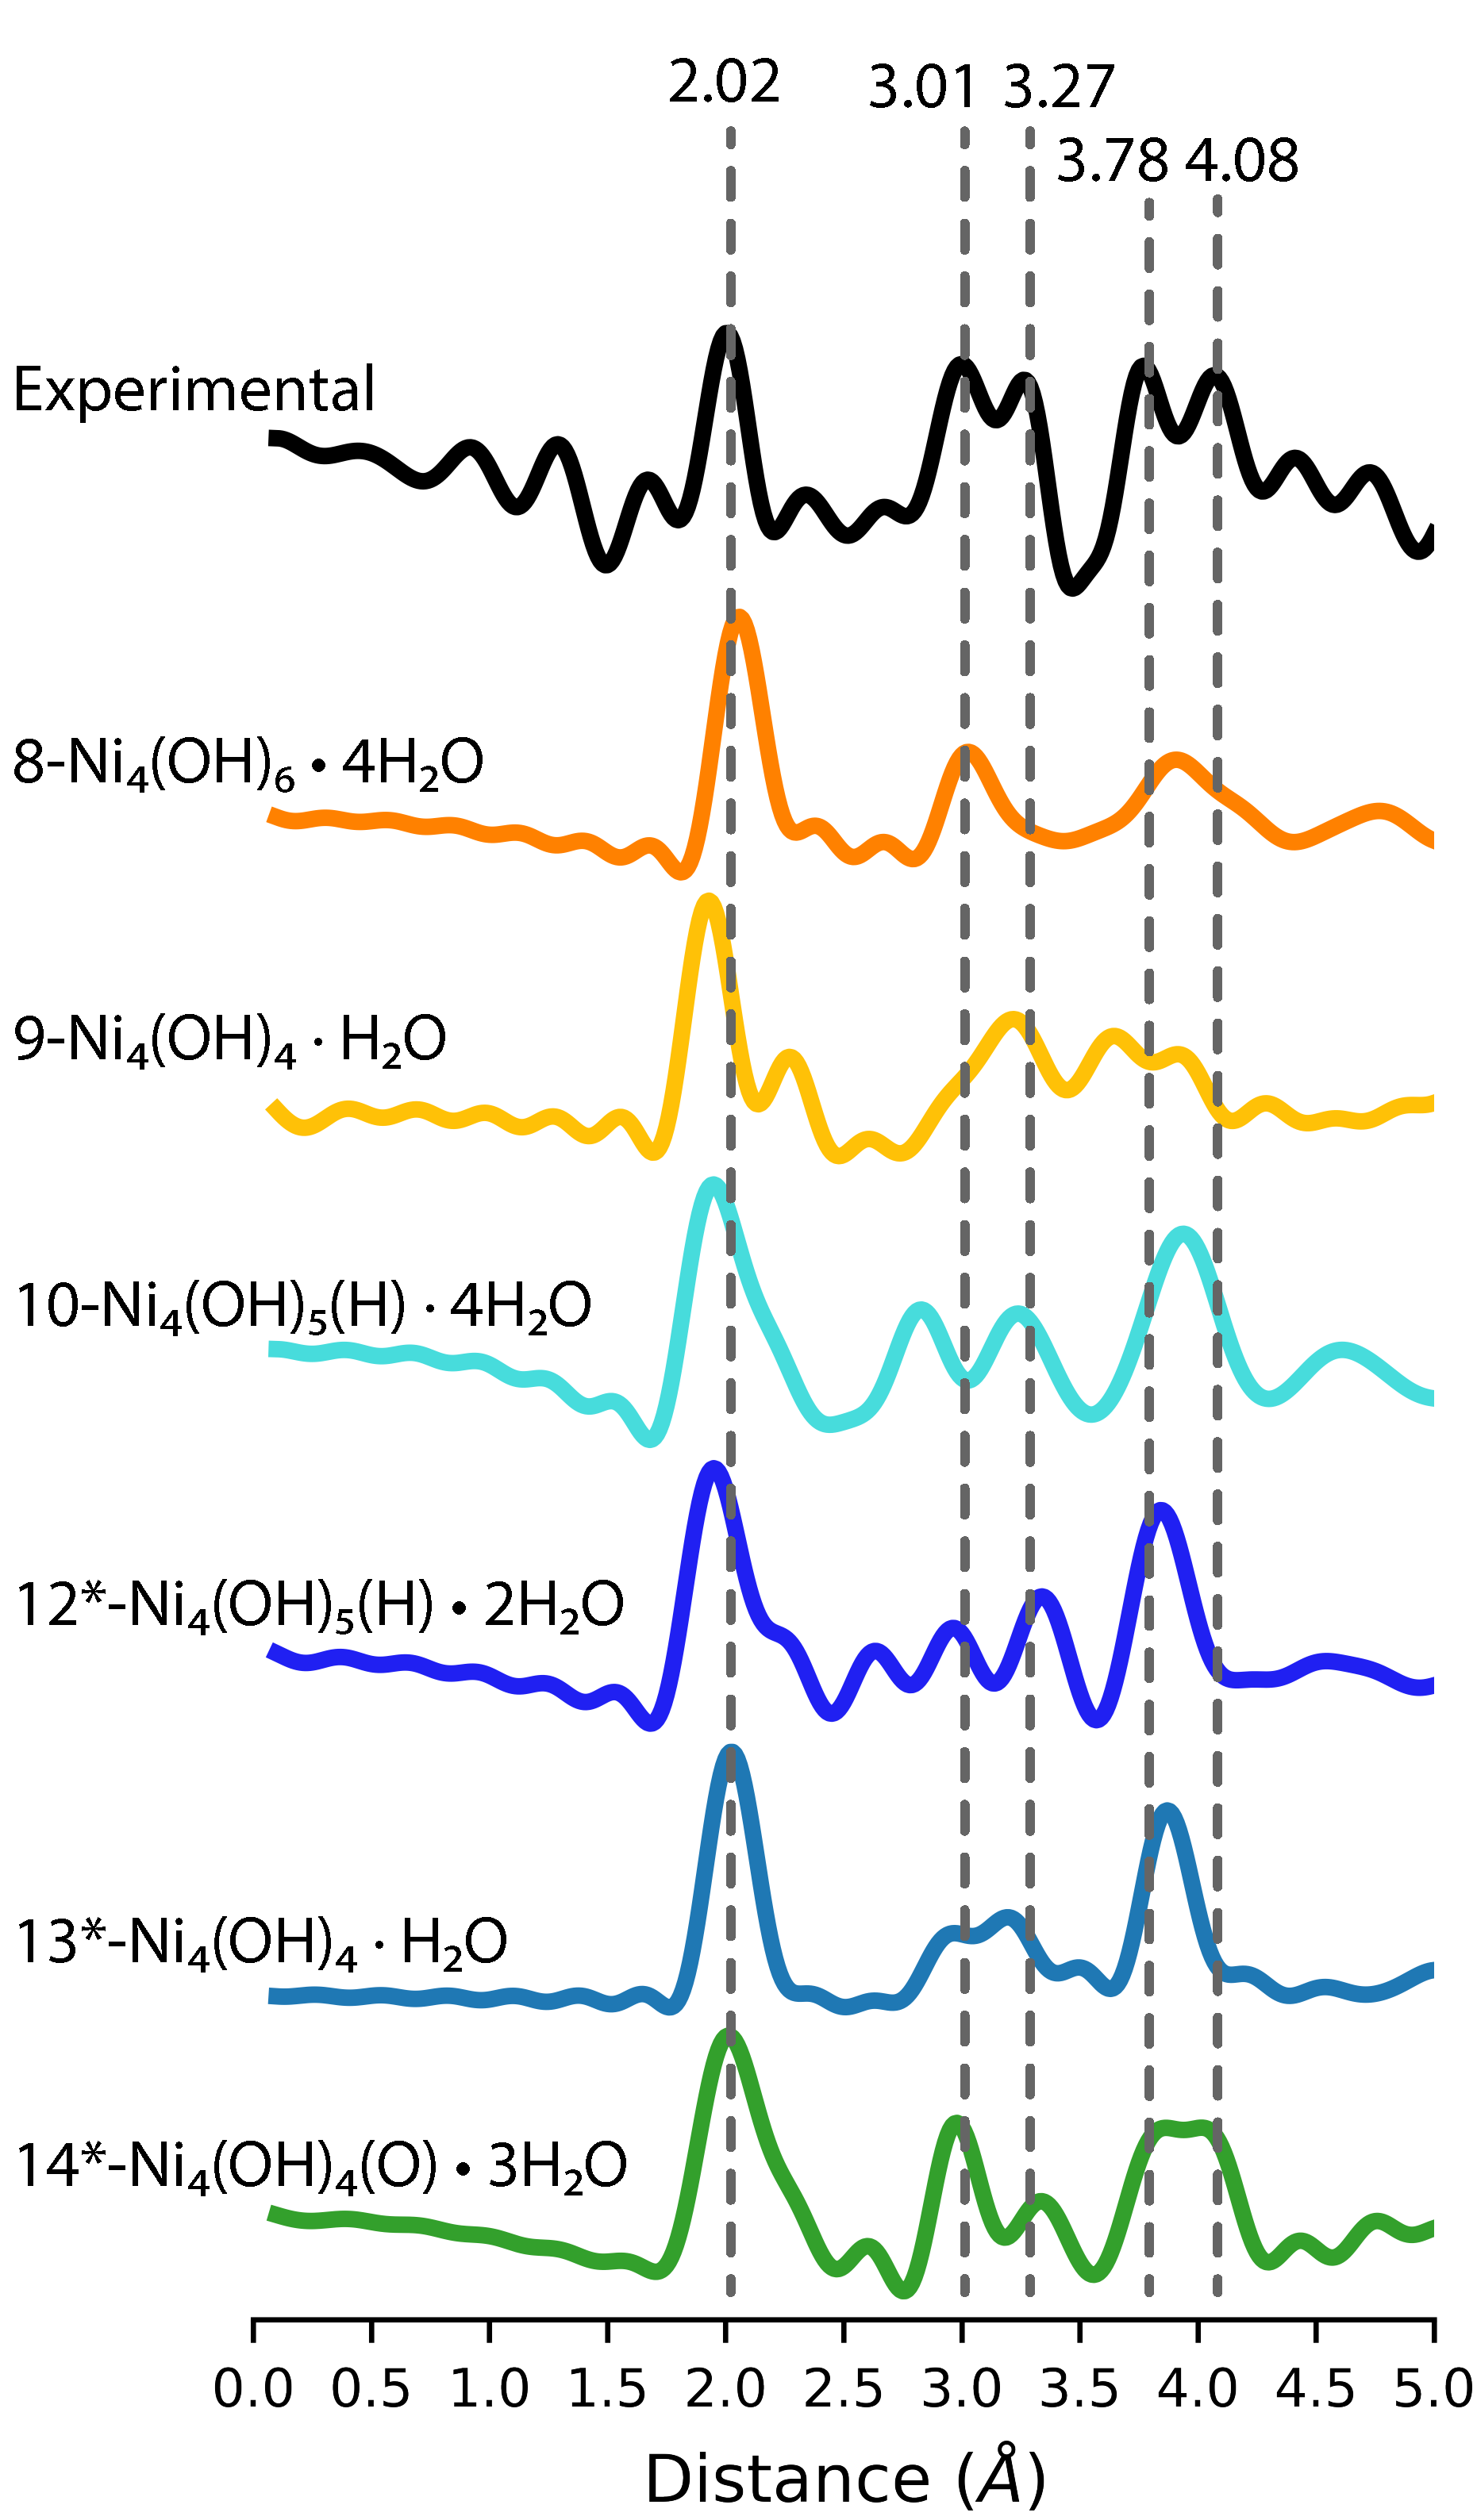
\includegraphics{zi-images/01-Ni-Graphics/2021-MAIN-single-dPDF-phase-diagram-select.png}
    \caption{
    Differential pair distribution functions (dPDFs) for all the structures present in Figure \ref{fig:Ni-structure-diagram-select}. The dPDFs consist of structures that are thermodynamic minima at higher \ce{H2O} partial pressure and structures that are selected based on their atomic distances that are not minima. The select structures are not thermodynamic minimum under any explored conditions and are denoted using a * (for example, 12*-\ce{Ni4(OH)5(H).2H2O} (royal)). Comparisons are made to the experimental dPDF by comparing the peak positions. 
    }
    \label{fig:dPDFs_TandP_trans_Ni-select}
\end{figure}

From \textit{ab initio} thermodynamic analysis, we find that 8-\ce{Ni4(OH)6.4H2O} (orange), 9-\ce{Ni4(OH)4.H2O} (yellow), and 10-\ce{Ni4(OH)5(H).4H2O} (teal) are thermodynamically relevant at elevated \ce{H2O} partial pressure ($P_{\text{\ce{H2O}}}=10^{0}$ bar as described by Figure \hl{XXXX} within the Supporting Information). 8-\ce{Ni4(OH)6.4H2O} (orange) is the reference structure during \textit{ab initio} thermodynamic analysis and features four \ce{H2O} coordinated to the center \ce{Ni} atoms with \ce{H2O} \hl{adsorption energies ranging from} X.XX to X.XX kJ mol$^{-1}$. The peak positions are within reason compared to the experimental structure, but do not recreate either of the \ce{Ni{\Compactcdots}Ni} or \ce{Ni{\Compactcdots}Zr} peak splitting. 9-\ce{Ni4(OH)4.H2O} (yellow) is analogous to 2-\ce{Ni4(OH)4} (blue) except that is also features a coordinated \ce{H2O}. Similar to 2-\ce{Ni4(OH)4} (blue), 9-\ce{Ni4(OH)4.H2O} (yellow) shows a \ce{Ni{\Compactcdots}Ni} peak at 2.42 {\AA} that is related to the distance of middle \ce{Ni} atoms (\ce{Ni} atoms away from the nodes). Additionally, 9-\ce{Ni4(OH)4.H2O} (yellow) shows \ce{Ni{\Compactcdots}Zr} peak splitting at lower atomic distances (3.66 {\AA} and 3.92 {\AA}). 10-\ce{Ni4(OH)5(H).4H2O} (teal) features only a single \ce{mu_{3}-OH} ligands removed. Therefore, we fail to observe the sharp \ce{Ni{\Compactcdots}Ni} peak at 2.29 {\AA} in this structure. 10-\ce{Ni4(OH)5(H).4H2O} (teal) slightly underpredicts the \ce{Ni-O} distance, features a shifted \ce{Ni{\Compactcdots}Ni} peak splitting, and contains a single \ce{Ni{\Compactcdots}Zr} peak. Interestingly, this structure features \ce{Ni-H} and adsorbed \ce{H2O} and two \ce{H2O}s that are uncoordinated to \ce{Ni} atoms within the cluster. These \ce{H2O}s interact with the organic linkers within the MOF framework, and contain \hl{adsorption energies} ranging from -130 kJ mol$^{-1}$ to -160 kJ mol$^{-1}$.

Our analysis finds the following non-thermodynamic minima structures, shown in Figure \ref{fig:Ni-structure-diagram}, to be relevant: 12*-\ce{Ni4(OH)5(H).2H2O} (royal), 13*-\ce{Ni4(OH)6.H2O} (blue), and 14*-\ce{Ni4(OH)4(O).3H2O} (green). Structure 12*-\ce{Ni4(OH)5(H).2H2O} (royal) structure features split \ce{Ni{\Compactcdots}Ni} peak that closely match the experimental dPDF, but also features another \ce{Ni{\Compactcdots}Ni} peak at 2.64 {\AA} and a broad \ce{Ni-O} peak. The 12*-\ce{Ni4(OH)5(H).2H2O} (royal) is the optimized structure of 8-\ce{Ni4(OH)5(H).4H2O} (teal) with 2 \ce{H2O} removed from the structure. The 2.64 {\AA} peak appears with the removal of the \ce{H2O}, suggesting the importance of the \ce{H2O} in the structure. Structure 13*-\ce{Ni4(OH)6.H2O} (blue) contains a sharp peak at 2.04 A related to the \ce{Ni-O} distance, \ce{Ni{\Compactcdots}Zr} splitting shifted to lower distances, and a single \ce{Ni{\Compactcdots}Zr} peak within the bounds of \ce{Ni{\Compactcdots}Zr} peak splitting. Structure 14*-\ce{Ni4(OH)4(O).3H2O} (green) are structurally unique because the cluster proton topology was modified by transforming a \ce{\mu_{2}-OH} ligand to an \ce{\mu_{2}-O} ligand. Although not as pronounced, 14*-\ce{Ni4(OH)4(O).3H2O} (green) demonstrates both \ce{Ni{\Compactcdots}Ni} and \ce{Ni{\Compactcdots}Zr} peak splitting. The upper bound for the \ce{Ni{\Compactcdots}Ni} peak is shifted 3.35 A from 3.27 A. The \ce{Ni-O} peak for 14*-\ce{Ni4(OH)4(O).3H2O} (green) matches the peak of 2.02 A of the experimental dPDF despite being noticeably broader. 

The structures in \ref{fig:Ni-structure-diagram-select} show much better agreement to the experimental dPDFs, which is supported by the higher coordination of the \ce{Ni} metal cluster. Although the structures appear at nonphysical \ce{H2O} partial pressure ($10^{0}$ bar) for the experimental system, our \textit{ab initio} thermodynamic analysis supports the idea of a high local \ce{H2O} chemical potential for the \ce{Ni} metal complex. The dPDF analysis for the modeling structures promotes a highly coordinated cluster as being more closely related to the experimental, which is only achieved at higher \ce{H2O} chemical potentials. 


% Old parts of this section. 
\begin{comment}

We focus on the dPDFS of structures 2-\ce{Ni4(OH)4} (blue), 7-\ce{Ni4(OH)4.H2O} (yellow), and 8-\ce{Ni4(OH)5(H).4H2O} (teal) (from Figure \ref{fig:phase_diagram_Ni_combined}). Structure 2-\ce{Ni4(OH)4} (blue) on both Figure \ref{fig:phase_diagram_Ni_combined} (a) and (b). Structurally, 2-\ce{Ni4(OH)4} (blue) shows a broad \ce{Ni{\Compactcdots}Ni} peak within the experimental bounds for \ce{Ni{\Compactcdots}Ni} peak splitting and feature a reasonable single \ce{Ni{\Compactcdots}Zr}. However, structure 2-\ce{Ni4(OH)4} (blue) underpredicts the \ce{Ni-O} distance by 0.11 {\AA} and features an additional peak at 2.29 {\AA} not seen in the experimental dPDF. We attribute the peak at 2.29 {\AA} to a \ce{Ni{\Compactcdots}Ni} distance that forms because of the loss of \ce{\mu_{3}-OH} ligands as \ce{H2O}. Similar to 2-\ce{Ni4(OH)4} (blue), we observe that structure 7-\ce{Ni4(OH)4.H2O} (yellow) also underpredicts the \ce{Ni-O} peak and shows the same \ce{Ni{\Compactcdots}Ni} peak at 2.29 {\AA}. Structure 7-\ce{Ni4(OH)4.H2O} (yellow) demonstrates peak \ce{Ni{\Compactcdots}Zr} peak splitting at distance shifted from the experimental \ce{Ni{\Compactcdots}Zr} peaks. The sharp \ce{Ni{\Compactcdots}Ni} peak around 2.29 {\AA} suggests that the experimental structure is not similar to structures 2-\ce{Ni4(OH)4} (blue) and 7-\ce{Ni4(OH)4.H2O} (yellow). 


Structure 8-\ce{Ni4(OH)5(H).4H2O} (teal) is different from structure 4-\ce{Ni4(OH)4} in that the structure features only a single \ce{mu_{3}-OH} ligands removed. Therefore, we fail to observe the sharp \ce{Ni{\Compactcdots}Ni} peak at 2.29 {\AA} in this structure. Structure 8-\ce{Ni4(OH)5(H).4H2O} (teal) slightly underpredicts the \ce{Ni-O} distance, features a shifted \ce{Ni{\Compactcdots}Ni} peak splitting, and contains a single \ce{Ni{\Compactcdots}Zr} peak. Interestingly, structure 8-\ce{Ni4(OH)5(H).4H2O} (teal) features \ce{Ni-H} and adsorbed \ce{H2O}. Structure 8-\ce{Ni4(OH)5(H).4H2O} (teal) also features two \ce{H2O}s that are uncoordinated to \ce{Ni} atoms within the cluster. These \ce{H2O}s interact with the organic linkers within the MOF framework, and contain adsorption energies ranging from -130 kJ mol$^{-1}$ to -160 kJ mol$^{-1}$.


    \begin{figure}[H]
        \centering
%        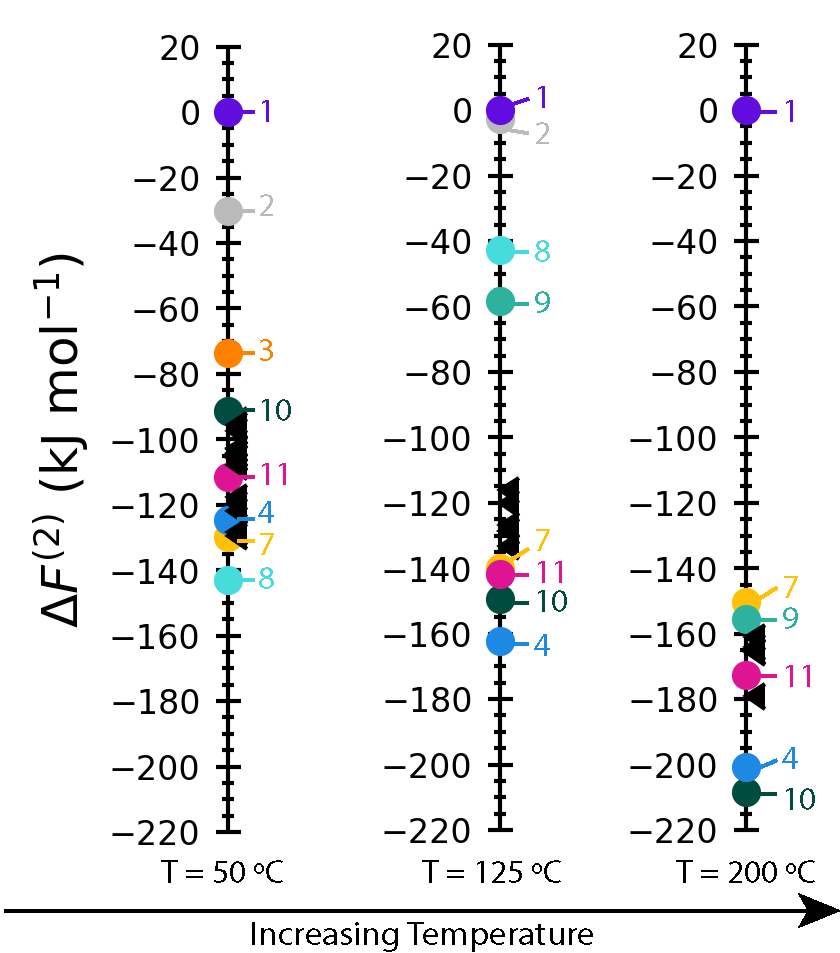
\includegraphics{zi-images/01-Ni-Graphics/2021-figure-lineplot.png}
        \caption{
        The $\Delta F^{(2)}(T,\mu_{\text{H}^{*}},\mu_{\text{OH}^{*}},N_{\text{Ni}^{*}})$ at a fixed \ce{H2} partial pressure of $10^{-5}$ bar and \ce{H2O} partial pressure     of $10^{-9}$ bar. As the temperature increases, the thermodynamic landscape within the structure library changes. The colored circles are classified as     thermodynamic minimum under some set of conditions, as described by Figure \ref{fig:phase_diagram_Ni_combined}. The colors and numbers are the same previously     utilized by Figure \ref{fig:Ni-structure-diagram} and Figure \ref{fig:phase_diagram_Ni_combined}. The black triangles highlight the free energy of a structure     within 50 kJ mol$^{-1}$ of the lowest energy structure at the specific set of conditions.
        }
        \label{fig:Ni-relative-energy-plot}
    \end{figure}
    
    Structures 14*-\ce{Ni4(OH)4(O).3H2O} (green), 13*-\ce{Ni4(OH)6.H2O} (blue), and \\ 12*-\ce{Ni4(OH)5(H).2H2O} (royal) do not appear on Figure     \ref{fig:phase_diagram_Ni_combined} because they do not represent a thermodynamic minimum under any of the conditions we explore. These structures are in competition with the other structures in the library. Therefore, we examine the full thermodynamic landscape at a fixed \ce{H2} partial pressure of $10^{-5}$ bar and \ce{H2O} partial pressure of $10^{-9}$ bar while varying the temperature in Figure \ref{fig:Ni-relative-energy-plot}. Additionally, we expand on the thermodynamic minimum in Figure \ref{fig:Ni-relative-energy-plot} to include library structures that are within 50 kJ mol$^{-1}$ of the lowest energy structure at those specific conditions. When considering additional structures within 50 kJ mol$^{-1}$, we determine the significance of the library and the potential for a distribution of active site structures at a specific reaction conditions. The closer in energy the structure is to the lowest energy structure, the more likely the active site is a distribution of active sites rather than the single lowest energy structure. 
\end{comment}



%%%%%%%%%%%%%%%%%%%%%%%%%%%%%%%%%%%%%%%%%%%%%%%%%%%%%%%%%%%%%%%%%%%%%
%% Discussion
%%%%%%%%%%%%%%%%%%%%%%%%%%%%%%%%%%%%%%%%%%%%%%%%%%%%%%%%%%%%%%%%%%%%
\newpage
\subsection{Discussion}
Our discussion focuses on the equilibrium thermodynamic structure resulting from exposure to \ce{H2} gas at different partial pressure and temperatures. The thermodynamic landscape of the \ce{Ni4}-cluster is presented in Figure \ref{fig:phase_diagram_Ni_combined}, and the model performance highlighted in Figure \ref{fig:dPDFs_TandP_trans_Ni}. We observe that the dPDFs for the structures shown in Figure \ref{fig:Ni-structure-diagram} diverge from the experimental dPDF with increased removal of \ce{H2O} and \ce{OH}-ligands as \ce{H2O}. Structures that exhibit a low \ce{Ni} coordination (such as 4-\ce{Ni2(H)2} (lilac)) contain peak positions that fail to match with the experimental peaks (Figure \ref{fig:dPDFs_TandP_trans_Ni}). Our results suggest that the presence of \ce{H2O} is vital in maintaining the correct dPDF peak positions and the \ce{Ni} coordination environment. The high coordination is maintained by the presence of \ce{OH}-ligands that link adjacent \ce{Ni} atoms and coordinated \ce{H2O}.

The structure that most resembles the experimental dPDF is 14*-\ce{Ni4(OH)4(O).3H2O} (green), but is not present as a thermodynamic minima during our thermodynamic modeling. 14*-\ce{Ni4(OH)4(O).3H2O} (green) matches the \ce{Ni-O} peak position, and demonstrates both \ce{Ni{\Compactcdots}Ni} and \ce{Ni{\Compactcdots}Zr} peak splitting. Structurally, 14*-\ce{Ni4(OH)4(O).3H2O} (green) features a \ce{\mu_{2}-O} that link adjacent \ce{Ni} atoms rather than the traditional \ce{\mu_{2}-OH} and features three coordinated \ce{H2O} species. The change in ligand environment helps create an asymmetric cluster. The bulk of the structures presented in Figures \ref{fig:Ni-structure-diagram} and \ref{fig:Ni-structure-diagram-select} are symmetric, but do not exhibit any peak splitting. Therefore, we suggest that the observed experimental peak splitting could be attributed to the asymmetry of the \ce{Ni} coordination environment. 

We evaluate the individual performance of model structures by comparing our results to the experimental dPDF from \citeauthor{PlateroPrats2017}. An important consideration for the experimental structure is that it could represent a distribution of \ce{Ni} metal complex structures. Our work only provides a snapshot of individual structures whereas the experimental dPDF could be comprised of a combination of these different structures.


Regardless, our observations that a high \ce{Ni} coordination environment 


The presence of \ce{H2O} within the active site structure is commonly debated. Experimentally, the temperature increase during activation (temperature ramp to and temperature hold at \SI{200}{Celsius} in the presence of \ce{H2})\hl{REFERENCE-ALL-TEMPERATURE RAMP PAPERS-Li-Sintering} is thought to remove any coordinated \ce{H2O} present within the active site. However, we find that structures containing \ce{H2O} more closely reasonable the experimental dPDF. Therefore, the presence of \ce{H2O} is vital for the \ce{Ni} cluster. If the increase is insufficient to remove all coordinated \ce{H2O}, then the necessary \ce{H2O} could remain within the structure. The transformation between \ce{OH} and \ce{H2O} could also explain the presence of \ce{H2O}. At ambient conditions, the cluster is primarily comprised of \ce{OH} ligands. At elevated temperatures, the \ce{OH} could be converted into strongly bound \ce{H2O}. As the temperature is cooled (for example back to \SI{50}{Celsius}), the \ce{OH} ligands would reform given the dynamic nature of the \ce{Ni} cluster. The interchange between \ce{OH} and \ce{H2O} under different reaction conditions is an important consideration and explains the presence of \ce{H2O} within the cluster. 



An important note is, by not considering the kinetics of these transformations, that our results only focus on the thermodynamic landscape. Our library of structures does not represent potential intermediate structures between different thermodynamic minima on the phase diagrams (Figure \ref{fig:phase_diagram_Ni_combined}). An alternate explanation for differences between modeling and experimental dPDFs is that the structure is kinetically limited rather than thermodynamically limited. Thermodynamically, Figure \ref{fig:phase_diagram_Ni_combined} suggests an active site structure that exhibits significant removal of \ce{OH}-ligands. Our analysis, however, does not consider the kinetic barriers associated for the removal of \ce{OH-ligands}. We assume that the kinetic barriers for the \ce{H2} adsorption and dissociation reaction are negligible, and fail to consider the barriers related to \ce{H2O} formation and dissociation. Computationally, \ce{H2} activation transition state barriers for \ce{OH} conversion to \ce{H2O} on a single \ce{Ni} atom reported by \citeauthor{Li2016sintering} are 180.7 kJ/mol,\cite{Li2016sintering} while \citeauthor{Shabbir2020} reports barriers only 61-70 kJ/mol.\cite{Shabbir2020} Our analysis reveals that the structures (Figure \ref{fig:Ni-structure-diagram-select} that best match the experimental dPDFs are structures with highly coordinated \ce{Ni} atoms. High \ce{Ni} coordination is only established via \ce{Ni-OH} bonds and coordinated \ce{H2O}. Therefore, we might infer that the cluster exists in a metastable state when exposed to \ce{H2} with the dominate structures determined by kinetic restraints rather than the thermodynamic minimum. The barriers involved in \ce{H2} dissociative adsorption or \ce{OH}-ligand removal could be sufficiently large to maintain the high \ce{Ni} coordination by presenting \ce{H2O} formation from the \ce{OH}-ligand. There could be metastable structure due to a kinetic barrier that matches the experimental dPDFs that we fail to consider. 






\begin{itemize}
    \item Discussion Topic 1: Presence of H2O 
    \begin{itemize}
        \item the conditions that the catalyst experiences, and how those conditions could be different.. and maybe discuss what the goals of those conditions are in terms of the structure of the catalyst
        \item \ce{Ni-H} formation in 8-\ce{Ni4(OH)5(H).4H2O} (teal).. how this structure generates the \ce{Ni-H} that everything thinks is the active species within the catalyst.
        \item 2-\ce{Ni4(OH)4} (blue) containing the \ce{Ni{\Compactcdots}} peak at 2-ish {\AA}.. dominates the phase space
        \item talk about what these results mean in the context of the activated structure and how the free energies of the structures are very similar in energy.
        \item talk about how, despite the additional \ce{Ni} species, only a single \ce{Ni} atom is the activated metal because structures.. we see that all the other structures are not in good agreement.. 
        \item Text: \\

        
        \hl{Both could actually be true? I don't think that these ideas are actually mutually exclusive here..}
        
        
        


    \end{itemize}
    \item Discussion Topic 2: Formate vs. Formate-Free \\
        \hl{Or... is is more like there is an important consideration that includes the nuclearity of the metal species??? are they mononuclear species bound to the node, or are they multinuclear species.. and are these species now regulated by whether or not formate is present within the cluster.}
        Another important consideration is the presence of formate (\ce{HCOO-}) species capping \ce{OH/H2O} ligand pairs of the MOF inorganic nodes. A recent publication by \citeauthor{Lu2020} determined that certain synthesis conditions lead to formate species capping \ce{OH/H2O} ligand pairs of the \ce{Zr-}based node.\cite{Lu2020} The \ce{OH/H2O} ligand pairs provide sites for anchoring \ce{Ni} species, which suggests that the metal cluster structure is dependent on the whether or not formate is present in the \ce{Zr-}based MOF structure. In a formate-free sample, metal grafting can occur on all four \ce{OH/H2O} ligands. However, with formate blocking three of four potential metal binding sites (\ce{OH/H2O} ligand pairs) the ALD process generates a multinuclear \ce{Ni} metal complex supported on NU-1000 that is observed within the small pore of NU-1000. Experimentally, a formate-free NU-1000 might generate a different distribution of \ce{Ni} active sites that is not considered by our model. Our model, which is derived from previous work by \citeauthor{Ye2017} and \citeauthor{PlateroPrats2017}, assumes the metal cluster is attached adjacent nodes within the small pore of NU-1000. All structural and compositions transformation begin from a structure containing four \ce{Ni} atoms. 
    \item Discussion Topic 3: Asymmetric STRUCTURES!!!!!! --> the asymmetric structures tend to have better agreement with the different peaks 
    \item Discussion Topic 4:
    
    \item Discussion Topic 1:
    \begin{itemize}
        \item Thermodynamically, active site formation does not demonstrate the formation of a \ce{Ni-H}, which is often to be the active species here. Possible explanation is that the dominate species here is not the \ce{Ni-H}. 
        \item The other explanation is that the \ce{Ni-H} could be the catalytically active site species; however, it might not be the lowest energy structure thermodynamically (meaning that it will not appear in on the phase diagram). There is a possibility that a distribution of active site structures exists, and that the active site structure that is catalytically active is not the dominate structure. 
        \item Additionally, something we did not consider was the \ce{H2} dissociation barriers onto \ce{Ni}. \citeauthor{Li2016sintering} demonstrate a barrier height for the transformation an \ce{OH}-site with \ce{H2} into a \ce{H}-site and \ce{H2O} of around 141 kJ/mol. Having such a high barrier is significant, and does suggest that kinetic limitations could also be present in our model. Our phase diagram is not able to capture, and include these kinetic limitations in the analysis. 
        \item Although we see the breakdown the cluster, kinetic barriers related to \ce{H2} adsorption and dissociation might inhibit the further breakdown of the cluster.
        \item Nonetheless, our model still provides clues into the potential active site structure of the 1-\ce{Ni4(OH)6} (purple) cluster. 
    \end{itemize}
    \item Discussion Topic 2:
    \begin{itemize}
        \item  Comparing the work from \citeauthor{PlateroPrats2017}, the majority of the structures contains under-coordinated \ce{Ni-atoms}. Experimentally, a coordination number of ~5 was observed.
        \item There are features shown on the phase diagram that are not present on the most recent, especially at high \ce{H2} partial pressures. At high \ce{H2} partial pressure, the structures start showing the presence of \ce{Ni-Ni} bonds. The peaks associated with \ce{Ni-Ni} bond formation are not seen experimentally, which suggests the cluster remains largely intact after activation. Throughout our analysis, as the cluster is reduced the formation is \ce{Ni-Ni} bonds is observed.     
        \item The dPDFs are from XRD data that is the average of ALL potential structures within the MOF framework.. the model dPDFs are snapshots of potential structures within the framework here. There is probably a distribution of active site structures that is dominated by the lowest energy structures. 
    \end{itemize}
    \item Discussion Topic 3: Rationalizing some of the experimental mkm work from Hafeera
    \begin{itemize}
        \item Could this help explain some of the discrepancies in reaction trends observed by \citeauthor{Shabbir2020} for \ce{Ni(II)} for \ce{C2H4} hydrogenation? The catalytically active site structure is the \ce{Ni-H} structure. However, thermodynamically, the formation of the \ce{Ni-H} is not dominate. Therefore, only a small number of sites are actually participating in the reaction. \hl{At least for Ni in Hafeera's work this could explain the differences in rates.}
        \item The influence of species such as formate being present on the node. Literature suggests that the reason a cluster forms, and why it forms within the c-pore, is because of the formate ligands capping the \ce{OH/H2O}-ligand pairs of the node. Comparing model and experimental clusters will depend on the experimental synthesis protocols. Only recently was the role of formate understood on the structure of the MOF node.  
    \end{itemize}
\end{itemize}

\newpage
\subsection{Conclusions}

%\begin{itemize}
%    \item The structural characteristics of the supported metal complexes are dependent on the reaction conditions.
%    \begin{itemize}
%        \item In the presence of a reducing agent (\ce{H2}), the hydroxo-ligands of the supported metal complexes are %removed (as \ce{H2O}). As previously suggested, we show computationally that \ce{H2} is important in breaking the %bonds between the metal clusters and the NU-1000 nodes. We provide the thermodynamic landscape for these %transformations.
%        \item Our findings show similar structural features and suggest that in an \ce{H2} reducing environment these %supported metal complexes containing \ce{OH}-ligands are not stable.  
%        \item At present, our modeling efforts demonstrate the formation of the more mobile \ce{M(0)} species. The breakdown %of the supported metal complex (removal of \ce{OH}-ligands within the cluster) reduces the metal atoms, thereby %generating the mobile \ce{M(0)} species.
%    \end{itemize}
%    \item A key question that still remains is whether these reduced supported metal complexes still exist as a combination %of NPs and multinuclear metal active sites or mononuclear active sites (single-sites) above \SI{200}{Celsius}.
%    \begin{itemize}
%        \item \citeauthor{Halder2020} determined that in an \ce{H2} environment the \ce{Cu3(OH)4} supported metal complexes %showed large \ce{Cu} NP formation. These particles were ~6.0 nm in diameter, which is larger than the ~3.0 nm %diameter hexagonal pore in NU-1000. Therefore, for \ce{Cu}-NU-1000 we know that these NPs grow, and we show using %our modeling that for \ce{Ni} we expect \ce{Ni} NPs to grow as well. 
%        \item Our present results support the experimental findings of \citeauthor{Halder2020} that reduced metal atoms are %generated. However, we extend the findings further and hypothesize that some of the single-site metal atoms remain %intact. Not all of the metal atoms are reduced to \ce{M(0)}; the metal atoms attached to the \ce{OH}-ligands of the %node remain. 
%        \item There are a few more additional calculations to be computed to test our theory (and these calculations are %currently being performed). The calculations contain two single-site models (with and without the \ce{M-H} species). %The metal atoms removed from the system will be accounted for as nanoclusters.
%    \end{itemize}
%\end{itemize}
%We have the following list of questions:
%\begin{itemize}
%    \item Experimentally, there is a different in the protocols to generate the single-site and the clusters in NU-1000? %Experimentally, you can differentiate between the two different catalysts in NU-1000? 
%    \item When looking at the Cu-NU-1000 discussion, did you ever remove the Cu-NPs and determine whether the framework that %was left behind was catalytically active? We wonder whether or not all the metal atoms are becoming the mobile \ce{M(0)} %species. 
%    \item The hexagonal pore returned to its original ~34 A value. How does the value of the pore compare when there are %single-site metal atoms attached to the node? 
%\end{itemize}

\subsection{References}

%The class makes various changes to the way that references are
%handled.  The class loads \textsf{natbib}, and also the
%appropriate bibliography style.  References can be made using
%the normal method; the citation should be placed before any
%punctuation, as the class will move it if using a superscript
%citation style
%\cite{Mena2000,Abernethy2003,Friedman-Hill2003,EuropeanCommission2008}.
%The use of \textsf{natbib} allows the use of the various citation
%commands of that package: \citeauthor{Abernethy2003} have shown
%something, in \citeyear{Cotton1999}, or as given by
%Ref.~\citenum{Mena2000}.  Long lists of authors will be
%automatically truncated in most article formats, but not in
%supplementary information or reviews \cite{Pople2003}. If you
%encounter problems with the citation macros, please check that
%your copy of \textsf{natbib} is up to date. The demonstration
%database file \texttt{achemso-demo.bib} shows how to complete
%entries correctly. Notice that ``\latin{et al.}'' is auto-formatted
%using the \texttt{\textbackslash latin} command.

%Multiple citations to be combined into a list can be %given as
%a single citation.  This uses the \textsf{mciteplus} %package
%\cite{Johnson1972,*Arduengo1992,*Eisenstein2005,*Arduengo%1994}.
%Citations other than the first of the list should be %indicated
%with a star. If the \textsf{mciteplus} package is not %installed,
%the standard bibliography tools will still work but %starred
%references will be ignored. Individual references can be %referred
%to using \texttt{\textbackslash mciteSubRef}:
%``ref.~\mciteSubRef{Eisenstein2005}''.

%The class also handles notes to be added to the bibliography.  These
%should be given in place in the document \bibnote{This is a note.
%The text will be moved the the references section.  The title of the
%section will change to ``Notes and References''.}.  As with
%citations, the text should be placed before punctuation.  A note is
%also generated if a citation has an optional note.  This assumes that
%the whole work has already been cited: odd numbering will result if
%this is not the case \cite[p.~1]{Cotton1999}.

%%%%%%%%%%%%%%%%%%%%%%%%%%%%%%%%%%%%%%%%%%%%%%%%%%%%%%%%%%%%%%%%%%%%%
%% The "Acknowledgement" section can be given in all manuscript
%% classes.  This should be given within the "acknowledgement"
%% environment, which will make the correct section or running title.
%%%%%%%%%%%%%%%%%%%%%%%%%%%%%%%%%%%%%%%%%%%%%%%%%%%%%%%%%%%%%%%%%%%%%
%\begin{acknowledgement}
%
%\hl{authors would like to thank \ldots''.
%
%The author thanks Mats Dahlgren for version one of \textsf{achemso},
%and Donald Arseneau for the code taken from \textsf{cite} to move
%citations after punctuation. Many users have provided feedback on the
%class, which is reflected in all of the different demonstrations
%shown in this document.}
%
%\end{acknowledgement}

%%%%%%%%%%%%%%%%%%%%%%%%%%%%%%%%%%%%%%%%%%%%%%%%%%%%%%%%%%%%%%%%%%%%%
%% The same is true for Supporting Information, which should use the
%% suppinfo environment.
%%%%%%%%%%%%%%%%%%%%%%%%%%%%%%%%%%%%%%%%%%%%%%%%%%%%%%%%%%%%%%%%%%%%%
%\begin{suppinfo}
%
%\hl{This will usually read something like: ``Experimental procedures and
%characterization data for all new compounds. The class will
%automatically add a sentence pointing to the information on-line:}
%
%\end{suppinfo}

%%%%%%%%%%%%%%%%%%%%%%%%%%%%%%%%%%%%%%%%%%%%%%%%%%%%%%%%%%%%%%%%%%%%%
%% The appropriate \bibliography command should be placed here.
%% Notice that the class file automatically sets \bibliographystyle
%% and also names the section correctly.
%%%%%%%%%%%%%%%%%%%%%%%%%%%%%%%%%%%%%%%%%%%%%%%%%%%%%%%%%%%%%%%%%%%%%
\newpage
\bibliography{achemso-demo}

\end{document}